% Options for packages loaded elsewhere
\PassOptionsToPackage{unicode}{hyperref}
\PassOptionsToPackage{hyphens}{url}
\documentclass[
]{article}
\usepackage{xcolor}
\usepackage[margin=1in]{geometry}
\usepackage{amsmath,amssymb}
\setcounter{secnumdepth}{-\maxdimen} % remove section numbering
\usepackage{iftex}
\ifPDFTeX
  \usepackage[T1]{fontenc}
  \usepackage[utf8]{inputenc}
  \usepackage{textcomp} % provide euro and other symbols
\else % if luatex or xetex
  \usepackage{unicode-math} % this also loads fontspec
  \defaultfontfeatures{Scale=MatchLowercase}
  \defaultfontfeatures[\rmfamily]{Ligatures=TeX,Scale=1}
\fi
\usepackage{lmodern}
\ifPDFTeX\else
  % xetex/luatex font selection
\fi
% Use upquote if available, for straight quotes in verbatim environments
\IfFileExists{upquote.sty}{\usepackage{upquote}}{}
\IfFileExists{microtype.sty}{% use microtype if available
  \usepackage[]{microtype}
  \UseMicrotypeSet[protrusion]{basicmath} % disable protrusion for tt fonts
}{}
\makeatletter
\@ifundefined{KOMAClassName}{% if non-KOMA class
  \IfFileExists{parskip.sty}{%
    \usepackage{parskip}
  }{% else
    \setlength{\parindent}{0pt}
    \setlength{\parskip}{6pt plus 2pt minus 1pt}}
}{% if KOMA class
  \KOMAoptions{parskip=half}}
\makeatother
\usepackage{color}
\usepackage{fancyvrb}
\newcommand{\VerbBar}{|}
\newcommand{\VERB}{\Verb[commandchars=\\\{\}]}
\DefineVerbatimEnvironment{Highlighting}{Verbatim}{commandchars=\\\{\}}
% Add ',fontsize=\small' for more characters per line
\usepackage{framed}
\definecolor{shadecolor}{RGB}{248,248,248}
\newenvironment{Shaded}{\begin{snugshade}}{\end{snugshade}}
\newcommand{\AlertTok}[1]{\textcolor[rgb]{0.94,0.16,0.16}{#1}}
\newcommand{\AnnotationTok}[1]{\textcolor[rgb]{0.56,0.35,0.01}{\textbf{\textit{#1}}}}
\newcommand{\AttributeTok}[1]{\textcolor[rgb]{0.13,0.29,0.53}{#1}}
\newcommand{\BaseNTok}[1]{\textcolor[rgb]{0.00,0.00,0.81}{#1}}
\newcommand{\BuiltInTok}[1]{#1}
\newcommand{\CharTok}[1]{\textcolor[rgb]{0.31,0.60,0.02}{#1}}
\newcommand{\CommentTok}[1]{\textcolor[rgb]{0.56,0.35,0.01}{\textit{#1}}}
\newcommand{\CommentVarTok}[1]{\textcolor[rgb]{0.56,0.35,0.01}{\textbf{\textit{#1}}}}
\newcommand{\ConstantTok}[1]{\textcolor[rgb]{0.56,0.35,0.01}{#1}}
\newcommand{\ControlFlowTok}[1]{\textcolor[rgb]{0.13,0.29,0.53}{\textbf{#1}}}
\newcommand{\DataTypeTok}[1]{\textcolor[rgb]{0.13,0.29,0.53}{#1}}
\newcommand{\DecValTok}[1]{\textcolor[rgb]{0.00,0.00,0.81}{#1}}
\newcommand{\DocumentationTok}[1]{\textcolor[rgb]{0.56,0.35,0.01}{\textbf{\textit{#1}}}}
\newcommand{\ErrorTok}[1]{\textcolor[rgb]{0.64,0.00,0.00}{\textbf{#1}}}
\newcommand{\ExtensionTok}[1]{#1}
\newcommand{\FloatTok}[1]{\textcolor[rgb]{0.00,0.00,0.81}{#1}}
\newcommand{\FunctionTok}[1]{\textcolor[rgb]{0.13,0.29,0.53}{\textbf{#1}}}
\newcommand{\ImportTok}[1]{#1}
\newcommand{\InformationTok}[1]{\textcolor[rgb]{0.56,0.35,0.01}{\textbf{\textit{#1}}}}
\newcommand{\KeywordTok}[1]{\textcolor[rgb]{0.13,0.29,0.53}{\textbf{#1}}}
\newcommand{\NormalTok}[1]{#1}
\newcommand{\OperatorTok}[1]{\textcolor[rgb]{0.81,0.36,0.00}{\textbf{#1}}}
\newcommand{\OtherTok}[1]{\textcolor[rgb]{0.56,0.35,0.01}{#1}}
\newcommand{\PreprocessorTok}[1]{\textcolor[rgb]{0.56,0.35,0.01}{\textit{#1}}}
\newcommand{\RegionMarkerTok}[1]{#1}
\newcommand{\SpecialCharTok}[1]{\textcolor[rgb]{0.81,0.36,0.00}{\textbf{#1}}}
\newcommand{\SpecialStringTok}[1]{\textcolor[rgb]{0.31,0.60,0.02}{#1}}
\newcommand{\StringTok}[1]{\textcolor[rgb]{0.31,0.60,0.02}{#1}}
\newcommand{\VariableTok}[1]{\textcolor[rgb]{0.00,0.00,0.00}{#1}}
\newcommand{\VerbatimStringTok}[1]{\textcolor[rgb]{0.31,0.60,0.02}{#1}}
\newcommand{\WarningTok}[1]{\textcolor[rgb]{0.56,0.35,0.01}{\textbf{\textit{#1}}}}
\usepackage{graphicx}
\makeatletter
\newsavebox\pandoc@box
\newcommand*\pandocbounded[1]{% scales image to fit in text height/width
  \sbox\pandoc@box{#1}%
  \Gscale@div\@tempa{\textheight}{\dimexpr\ht\pandoc@box+\dp\pandoc@box\relax}%
  \Gscale@div\@tempb{\linewidth}{\wd\pandoc@box}%
  \ifdim\@tempb\p@<\@tempa\p@\let\@tempa\@tempb\fi% select the smaller of both
  \ifdim\@tempa\p@<\p@\scalebox{\@tempa}{\usebox\pandoc@box}%
  \else\usebox{\pandoc@box}%
  \fi%
}
% Set default figure placement to htbp
\def\fps@figure{htbp}
\makeatother
\setlength{\emergencystretch}{3em} % prevent overfull lines
\providecommand{\tightlist}{%
  \setlength{\itemsep}{0pt}\setlength{\parskip}{0pt}}
\usepackage{bookmark}
\IfFileExists{xurl.sty}{\usepackage{xurl}}{} % add URL line breaks if available
\urlstyle{same}
\hypersetup{
  hidelinks,
  pdfcreator={LaTeX via pandoc}}

\author{}
\date{\vspace{-2.5em}}

\begin{document}

\begin{Shaded}
\begin{Highlighting}[]
\NormalTok{df\_doctored }\OtherTok{\textless{}{-}}\NormalTok{ df }\SpecialCharTok{\%\textgreater{}\%}
  \FunctionTok{filter}\NormalTok{((ticker }\SpecialCharTok{!=} \StringTok{"NFLX"} \SpecialCharTok{|}\NormalTok{ call\_put }\SpecialCharTok{!=} \StringTok{"calls"}\NormalTok{) }\SpecialCharTok{|}\NormalTok{ (K }\SpecialCharTok{\textless{}} \DecValTok{266} \SpecialCharTok{\&}\NormalTok{ true\_price }\SpecialCharTok{\textless{}} \DecValTok{400}\NormalTok{)) }\SpecialCharTok{\%\textgreater{}\%}
  \FunctionTok{filter}\NormalTok{((ticker }\SpecialCharTok{!=} \StringTok{"NVDA"} \SpecialCharTok{|}\NormalTok{ call\_put }\SpecialCharTok{!=} \StringTok{"calls"}\NormalTok{) }\SpecialCharTok{|}\NormalTok{ (K }\SpecialCharTok{\textless{}} \DecValTok{500} \SpecialCharTok{\&}\NormalTok{ true\_price }\SpecialCharTok{\textless{}} \DecValTok{300}\NormalTok{)) }\SpecialCharTok{\%\textgreater{}\%}
  \FunctionTok{filter}\NormalTok{((ticker }\SpecialCharTok{!=} \StringTok{"NFLX"} \SpecialCharTok{|}\NormalTok{ call\_put }\SpecialCharTok{!=} \StringTok{"puts"}\NormalTok{) }\SpecialCharTok{|}\NormalTok{ (K }\SpecialCharTok{\textless{}} \DecValTok{266} \SpecialCharTok{\&}\NormalTok{ (K }\SpecialCharTok{\textless{}} \DecValTok{100} \SpecialCharTok{|}\NormalTok{ true\_price }\SpecialCharTok{\textgreater{}} \DecValTok{10}\NormalTok{))) }\SpecialCharTok{\%\textgreater{}\%}
  \FunctionTok{filter}\NormalTok{((ticker }\SpecialCharTok{!=} \StringTok{"NVDA"} \SpecialCharTok{|}\NormalTok{ call\_put }\SpecialCharTok{!=} \StringTok{"puts"}\NormalTok{) }\SpecialCharTok{|}\NormalTok{ (K }\SpecialCharTok{\textless{}} \DecValTok{500} \SpecialCharTok{\&}\NormalTok{ (K }\SpecialCharTok{\textless{}} \DecValTok{300} \SpecialCharTok{|}\NormalTok{ true\_price }\SpecialCharTok{\textgreater{}} \DecValTok{100}\NormalTok{)))}

\NormalTok{df }\OtherTok{\textless{}{-}}\NormalTok{ df\_doctored}
\end{Highlighting}
\end{Shaded}

\section{Regresní analýza}\label{regresnuxed-analuxfdza}

\subsection{Absolutní}\label{absolutnuxed}

\begin{Shaded}
\begin{Highlighting}[]
\NormalTok{df\_absolute }\OtherTok{\textless{}{-}}\NormalTok{ df\_doctored }\SpecialCharTok{\%\textgreater{}\%}
  \FunctionTok{pivot\_longer}\NormalTok{(}\AttributeTok{cols =} \FunctionTok{c}\NormalTok{(user\_bs, user\_crr, user\_mc),}
               \AttributeTok{names\_to =} \StringTok{"model"}\NormalTok{,}
               \AttributeTok{values\_to =} \StringTok{"model\_price"}\NormalTok{) }\SpecialCharTok{\%\textgreater{}\%}
  \CommentTok{\#filter(model == "user\_crr") \%\textgreater{}\%}
  \FunctionTok{mutate}\NormalTok{(}\AttributeTok{pricing\_error =}\NormalTok{ true\_price }\SpecialCharTok{{-}}\NormalTok{ model\_price) }\SpecialCharTok{\%\textgreater{}\%}
  \FunctionTok{filter}\NormalTok{(}\FunctionTok{is.finite}\NormalTok{(pricing\_error)) }\SpecialCharTok{\%\textgreater{}\%}
  \CommentTok{\#filter(abs(pricing\_error) \textless{}= 13) \%\textgreater{}\%}
  \FunctionTok{mutate}\NormalTok{(}\AttributeTok{snapshot\_date =} \FunctionTok{as.Date}\NormalTok{(expiration) }\SpecialCharTok{{-}} \FunctionTok{round}\NormalTok{(T }\SpecialCharTok{*} \DecValTok{365}\NormalTok{)) }\SpecialCharTok{\%\textgreater{}\%}
  \FunctionTok{mutate}\NormalTok{(}\AttributeTok{snapshot\_month =} \FunctionTok{format}\NormalTok{(snapshot\_date, }\StringTok{"\%m"}\NormalTok{))}
\end{Highlighting}
\end{Shaded}

\begin{Shaded}
\begin{Highlighting}[]
\NormalTok{df\_absolute\_temp }\OtherTok{\textless{}{-}}\NormalTok{ df\_absolute }\CommentTok{\#\%\textgreater{}\% filter(am\_eu == "american" \& call\_put == "calls")}
\NormalTok{train\_indexes }\OtherTok{\textless{}{-}} \FunctionTok{sample}\NormalTok{(}\DecValTok{1}\SpecialCharTok{:}\FunctionTok{nrow}\NormalTok{(df\_absolute\_temp), }\AttributeTok{size =} \FloatTok{0.8} \SpecialCharTok{*} \FunctionTok{nrow}\NormalTok{(df\_absolute\_temp))}

\NormalTok{train\_data\_abs }\OtherTok{\textless{}{-}}\NormalTok{ df\_absolute\_temp[train\_indexes, ]}
\NormalTok{test\_data\_abs }\OtherTok{\textless{}{-}}\NormalTok{ df\_absolute\_temp[}\SpecialCharTok{{-}}\NormalTok{train\_indexes, ]}
\end{Highlighting}
\end{Shaded}

\subsubsection{Prostý model}\label{prostuxfd-model}

\begin{Shaded}
\begin{Highlighting}[]
\NormalTok{subset\_args }\OtherTok{\textless{}{-}} \FunctionTok{c}\NormalTok{(}
  \StringTok{"S"}\NormalTok{,}
  \StringTok{"moneyness"}\NormalTok{,}
  \StringTok{"K"}\NormalTok{,}
  \StringTok{"r"}\NormalTok{,}
  \StringTok{"sigma"}\NormalTok{,}
  \StringTok{"q"}\NormalTok{,}
  \StringTok{"T"}\NormalTok{,}
  \CommentTok{\#"am\_eu",}
  \StringTok{"call\_put"}\NormalTok{,}
  \CommentTok{\#"model",}
  \StringTok{"ticker"}\NormalTok{,}
  \StringTok{"snapshot\_month"}
\NormalTok{  )}
\NormalTok{interactions }\OtherTok{\textless{}{-}} \FunctionTok{c}\NormalTok{(}
  \CommentTok{\#"q:am\_eu",}
\NormalTok{)}

\NormalTok{rhs }\OtherTok{\textless{}{-}} \FunctionTok{paste}\NormalTok{(}\FunctionTok{c}\NormalTok{(subset\_args, interactions), }\AttributeTok{collapse =} \StringTok{" + "}\NormalTok{)}
\NormalTok{formula }\OtherTok{\textless{}{-}} \FunctionTok{as.formula}\NormalTok{(}\FunctionTok{paste}\NormalTok{(}\StringTok{"pricing\_error \textasciitilde{} "}\NormalTok{, rhs))}
\CommentTok{\#T\_crr \textless{}{-} lm(pricing\_error \textasciitilde{} T + as.factor(snapshot\_month), data = train\_data)}
\NormalTok{regression\_absolute }\OtherTok{\textless{}{-}} \FunctionTok{lm}\NormalTok{(formula, }\AttributeTok{data =}\NormalTok{ train\_data\_abs)}

\FunctionTok{summary}\NormalTok{(regression\_absolute)}
\end{Highlighting}
\end{Shaded}

\begin{verbatim}
## 
## Call:
## lm(formula = formula, data = train_data_abs)
## 
## Residuals:
##     Min      1Q  Median      3Q     Max 
## -926.59   -2.00    1.61    5.69  994.81 
## 
## Coefficients:
##                    Estimate Std. Error t value Pr(>|t|)    
## (Intercept)       2.493e+01  3.774e+00   6.607 3.93e-11 ***
## S                -3.750e-02  1.185e-03 -31.639  < 2e-16 ***
## moneyness         7.988e-02  6.829e-03  11.697  < 2e-16 ***
## K                 1.386e-02  2.581e-04  53.685  < 2e-16 ***
## r                 8.779e+02  5.542e+01  15.842  < 2e-16 ***
## sigma            -5.146e+00  2.172e+00  -2.369   0.0178 *  
## q                -7.074e+02  9.861e+01  -7.173 7.33e-13 ***
## T                 1.506e+00  8.062e-02  18.681  < 2e-16 ***
## call_putputs      3.113e+00  1.138e-01  27.342  < 2e-16 ***
## ticker^VIX       -5.444e+01  4.351e+00 -12.513  < 2e-16 ***
## ticker^XDA       -5.793e+01  4.974e+00 -11.648  < 2e-16 ***
## ticker^XDB       -5.620e+01  4.310e+00 -13.040  < 2e-16 ***
## ticker^XDE       -5.646e+01  3.735e+00 -15.117  < 2e-16 ***
## ticker^XDN       -5.668e+01  4.088e+00 -13.863  < 2e-16 ***
## tickerAAPL       -5.024e+01  2.904e+00 -17.303  < 2e-16 ***
## tickerAMD        -5.212e+01  3.138e+00 -16.609  < 2e-16 ***
## tickerAMZN       -5.284e+01  2.975e+00 -17.761  < 2e-16 ***
## tickerGOOGL      -4.486e+01  2.847e+00 -15.760  < 2e-16 ***
## tickerJNJ        -3.045e+01  4.270e+00  -7.132 9.89e-13 ***
## tickerKO         -3.612e+01  4.150e+00  -8.704  < 2e-16 ***
## tickerMETA       -4.519e+01  2.543e+00 -17.774  < 2e-16 ***
## tickerMSFT       -4.560e+01  2.772e+00 -16.454  < 2e-16 ***
## tickerNFLX       -5.807e+01  3.133e+00 -18.532  < 2e-16 ***
## tickerNVDA       -5.270e+01  3.071e+00 -17.157  < 2e-16 ***
## tickerPG         -3.620e+01  3.894e+00  -9.297  < 2e-16 ***
## tickerTSLA       -5.213e+01  2.939e+00 -17.737  < 2e-16 ***
## snapshot_month02  1.493e-01  1.654e-01   0.903   0.3667    
## snapshot_month03 -1.537e-01  1.843e-01  -0.834   0.4042    
## snapshot_month05  2.765e+00  2.244e-01  12.321  < 2e-16 ***
## ---
## Signif. codes:  0 '***' 0.001 '**' 0.01 '*' 0.05 '.' 0.1 ' ' 1
## 
## Residual standard error: 34.28 on 375333 degrees of freedom
## Multiple R-squared:  0.01882,    Adjusted R-squared:  0.01875 
## F-statistic: 257.2 on 28 and 375333 DF,  p-value: < 2.2e-16
\end{verbatim}

\subsubsection{Předpoklady}\label{pux159edpoklady}

Kontrola normality dat:

\begin{Shaded}
\begin{Highlighting}[]
\FunctionTok{png}\NormalTok{(}\StringTok{"\textasciitilde{}/Praxe/bakalarka/figures/hist\_absolute.png"}\NormalTok{, }\AttributeTok{width =} \DecValTok{6}\NormalTok{, }\AttributeTok{height =} \DecValTok{4}\NormalTok{, }\AttributeTok{units =} \StringTok{"in"}\NormalTok{, }\AttributeTok{res =} \DecValTok{300}\NormalTok{)}
\NormalTok{histogram\_abs }\OtherTok{\textless{}{-}} \FunctionTok{hist}\NormalTok{(df\_absolute\_temp}\SpecialCharTok{$}\NormalTok{pricing\_error, }\AttributeTok{breaks =} \DecValTok{100}\NormalTok{)}
\FunctionTok{dev.off}\NormalTok{()}
\end{Highlighting}
\end{Shaded}

\begin{verbatim}
## png 
##   2
\end{verbatim}

\begin{Shaded}
\begin{Highlighting}[]
\NormalTok{histogram\_abs}
\end{Highlighting}
\end{Shaded}

\begin{verbatim}
## $breaks
##  [1] -960 -940 -920 -900 -880 -860 -840 -820 -800 -780 -760 -740 -720 -700 -680
## [16] -660 -640 -620 -600 -580 -560 -540 -520 -500 -480 -460 -440 -420 -400 -380
## [31] -360 -340 -320 -300 -280 -260 -240 -220 -200 -180 -160 -140 -120 -100  -80
## [46]  -60  -40  -20    0   20   40   60   80  100  120  140  160  180  200  220
## [61]  240  260  280  300  320  340  360  380  400  420  440  460  480  500  520
## [76]  540  560  580  600  620  640  660  680  700  720  740  760  780  800  820
## [91]  840  860  880  900  920  940  960  980 1000
## 
## $counts
##  [1]      6      0      0      3      0      0      3      0      0      6
## [11]     15      3     21     12      3     27     13     29     15     27
## [21]     51     39     33     18     36     33     58     65     61    112
## [31]    112     93     96    120    143    240    197    268    322    555
## [41]    441    824   1375   1497   2823   5189  13693 118267 300957  12942
## [51]   3972   1879    956    567    297    116    127     95     21     24
## [61]     39      0     17      5     17     21     18      0      6      3
## [71]      6      0      6     15      3      3      9     24      3     19
## [81]      5      0      6      9      7     12     12      8      8      7
## [91]      0      0      0      0      3     12      0      3
## 
## $density
##  [1] 6.393821e-07 0.000000e+00 0.000000e+00 3.196911e-07 0.000000e+00
##  [6] 0.000000e+00 3.196911e-07 0.000000e+00 0.000000e+00 6.393821e-07
## [11] 1.598455e-06 3.196911e-07 2.237837e-06 1.278764e-06 3.196911e-07
## [16] 2.877219e-06 1.385328e-06 3.090347e-06 1.598455e-06 2.877219e-06
## [21] 5.434748e-06 4.155984e-06 3.516602e-06 1.918146e-06 3.836293e-06
## [26] 3.516602e-06 6.180694e-06 6.926639e-06 6.500385e-06 1.193513e-05
## [31] 1.193513e-05 9.910423e-06 1.023011e-05 1.278764e-05 1.523861e-05
## [36] 2.557528e-05 2.099305e-05 2.855907e-05 3.431351e-05 5.914284e-05
## [41] 4.699458e-05 8.780848e-05 1.465251e-04 1.595258e-04 3.008293e-04
## [46] 5.529590e-04 1.459177e-03 1.260297e-02 3.207109e-02 1.379147e-03
## [51] 4.232710e-04 2.002332e-04 1.018749e-04 6.042161e-05 3.164941e-05
## [56] 1.236139e-05 1.353359e-05 1.012355e-05 2.237837e-06 2.557528e-06
## [61] 4.155984e-06 0.000000e+00 1.811583e-06 5.328184e-07 1.811583e-06
## [66] 2.237837e-06 1.918146e-06 0.000000e+00 6.393821e-07 3.196911e-07
## [71] 6.393821e-07 0.000000e+00 6.393821e-07 1.598455e-06 3.196911e-07
## [76] 3.196911e-07 9.590732e-07 2.557528e-06 3.196911e-07 2.024710e-06
## [81] 5.328184e-07 0.000000e+00 6.393821e-07 9.590732e-07 7.459458e-07
## [86] 1.278764e-06 1.278764e-06 8.525095e-07 8.525095e-07 7.459458e-07
## [91] 0.000000e+00 0.000000e+00 0.000000e+00 0.000000e+00 3.196911e-07
## [96] 1.278764e-06 0.000000e+00 3.196911e-07
## 
## $mids
##  [1] -950 -930 -910 -890 -870 -850 -830 -810 -790 -770 -750 -730 -710 -690 -670
## [16] -650 -630 -610 -590 -570 -550 -530 -510 -490 -470 -450 -430 -410 -390 -370
## [31] -350 -330 -310 -290 -270 -250 -230 -210 -190 -170 -150 -130 -110  -90  -70
## [46]  -50  -30  -10   10   30   50   70   90  110  130  150  170  190  210  230
## [61]  250  270  290  310  330  350  370  390  410  430  450  470  490  510  530
## [76]  550  570  590  610  630  650  670  690  710  730  750  770  790  810  830
## [91]  850  870  890  910  930  950  970  990
## 
## $xname
## [1] "df_absolute_temp$pricing_error"
## 
## $equidist
## [1] TRUE
## 
## attr(,"class")
## [1] "histogram"
\end{verbatim}

Data jsou normálně rozložená s velmi silnými ohony a slabě negativním
sklonem.

Celková kontrola regresního modelu:

\begin{Shaded}
\begin{Highlighting}[]
\FunctionTok{png}\NormalTok{(}\StringTok{"\textasciitilde{}/Praxe/bakalarka/figures/basic\_lm\_plots.png"}\NormalTok{, }\AttributeTok{width =} \DecValTok{6}\NormalTok{, }\AttributeTok{height =} \DecValTok{4}\NormalTok{, }\AttributeTok{units =} \StringTok{"in"}\NormalTok{, }\AttributeTok{res =} \DecValTok{300}\NormalTok{)}
\FunctionTok{par}\NormalTok{(}\AttributeTok{mfrow =} \FunctionTok{c}\NormalTok{(}\DecValTok{2}\NormalTok{, }\DecValTok{2}\NormalTok{))}
\FunctionTok{plot}\NormalTok{(regression\_absolute)}
\FunctionTok{dev.off}\NormalTok{()}
\end{Highlighting}
\end{Shaded}

\begin{verbatim}
## png 
##   2
\end{verbatim}

\begin{Shaded}
\begin{Highlighting}[]
\FunctionTok{par}\NormalTok{(}\AttributeTok{mfrow =} \FunctionTok{c}\NormalTok{(}\DecValTok{2}\NormalTok{, }\DecValTok{2}\NormalTok{))}
\FunctionTok{plot}\NormalTok{(regression\_absolute)}
\end{Highlighting}
\end{Shaded}

\pandocbounded{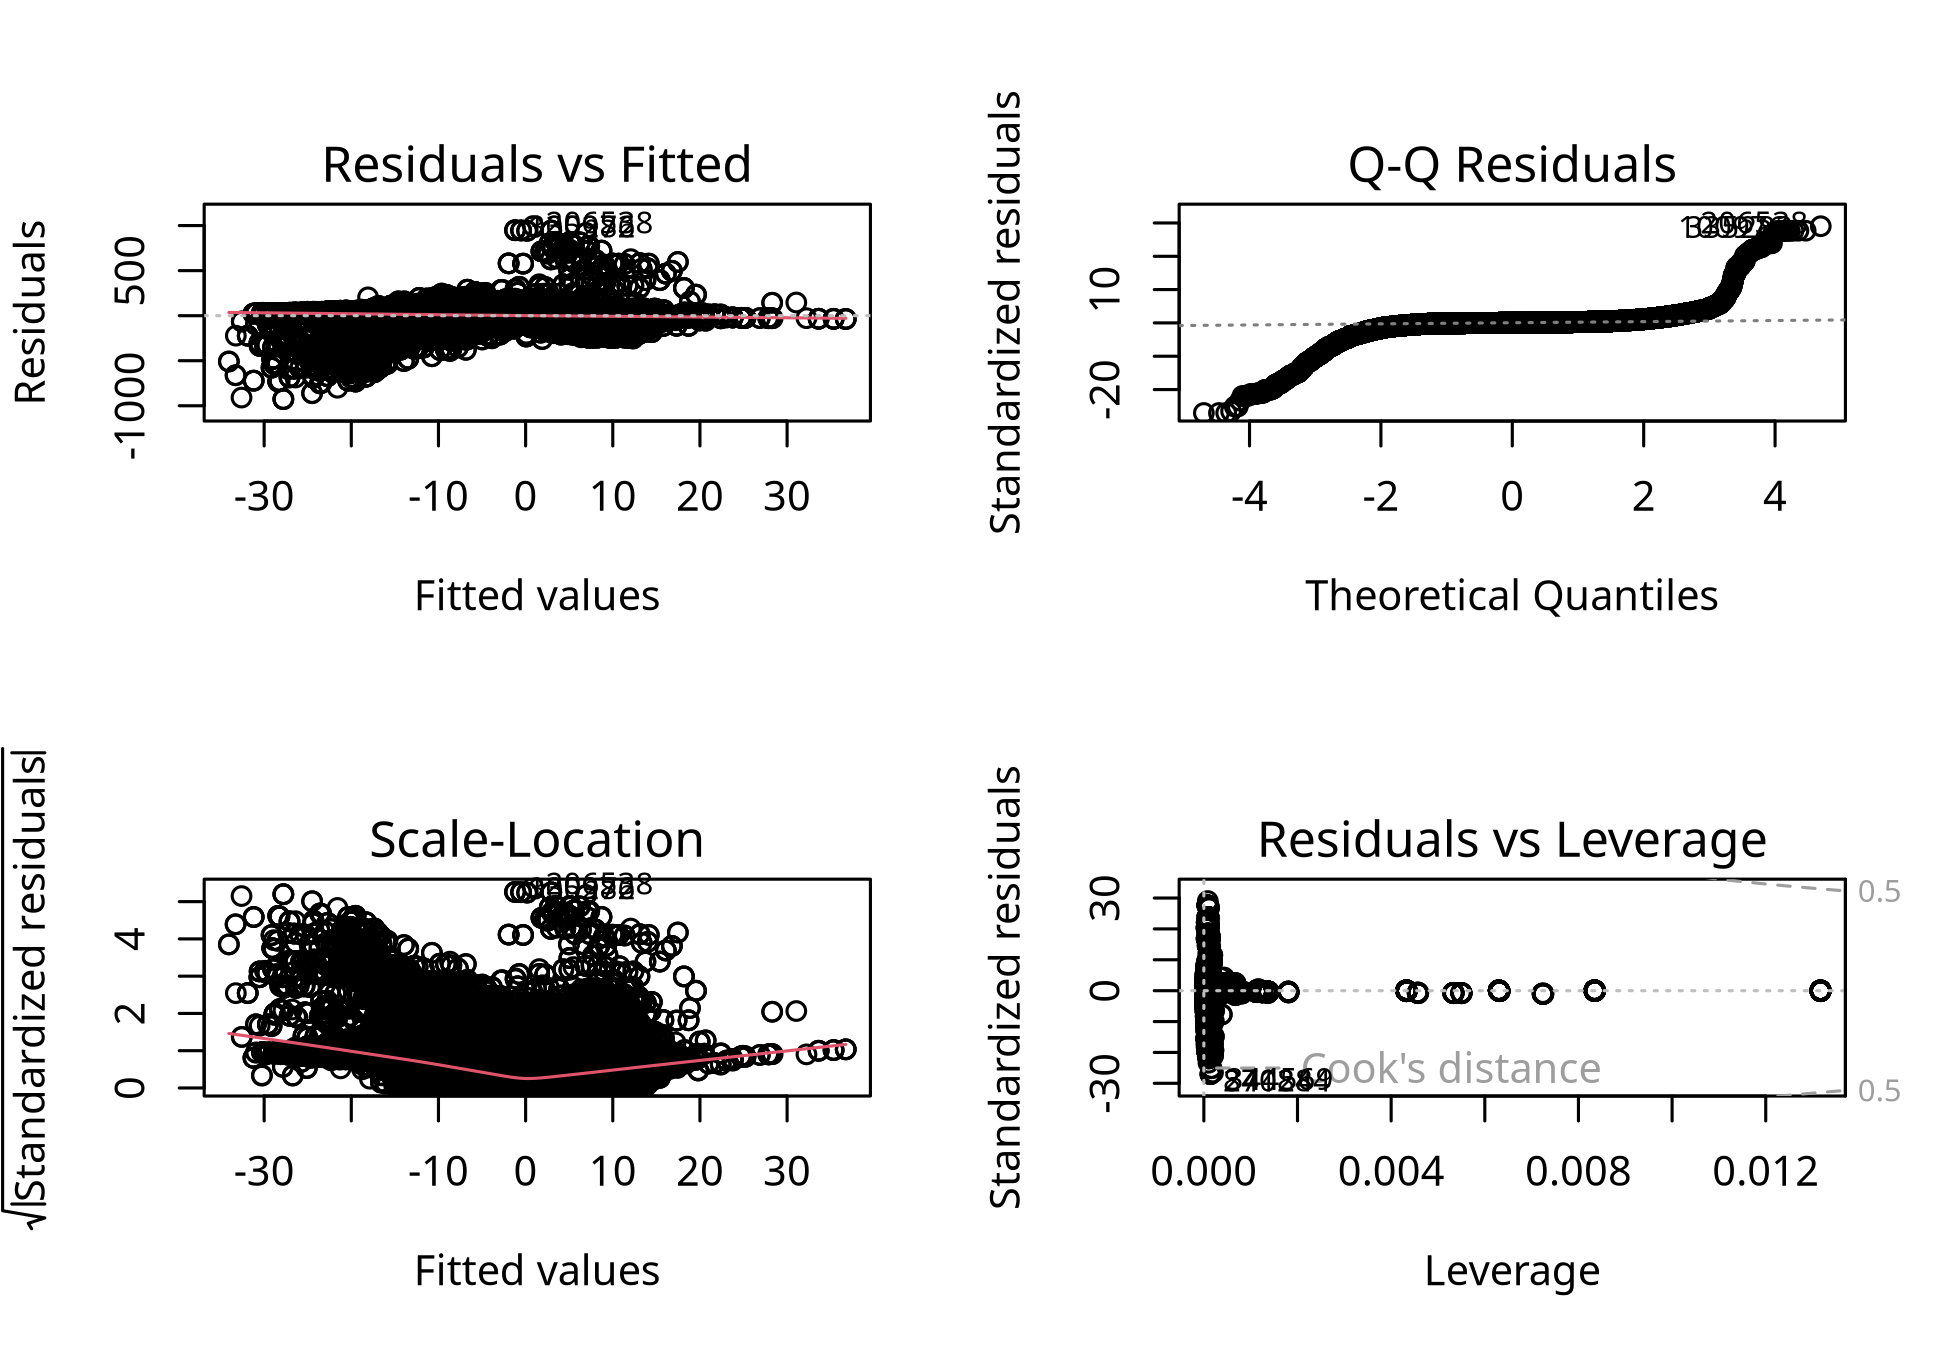
\includegraphics[keepaspectratio]{regression_files/regression_files/figure-latex/bm_tests-1.png}}

\begin{Shaded}
\begin{Highlighting}[]
\FunctionTok{par}\NormalTok{(}\AttributeTok{mfrow =} \FunctionTok{c}\NormalTok{(}\DecValTok{1}\NormalTok{, }\DecValTok{1}\NormalTok{))}
\end{Highlighting}
\end{Shaded}

První graf ukazuje lineární funkci, ne konstantní funkci. Co to přesně
znamená? QQ-plot (graf 2) potvrzuje přiměřeně vhodné rozdělení dat.
Homoskedasticita silně porušena (graf 3). Cookovy vzdálenosti (graf 4)
jsou ok.

Druhá kontrola homoscedasticity:

\begin{Shaded}
\begin{Highlighting}[]
\FunctionTok{bptest}\NormalTok{(regression\_absolute)}
\end{Highlighting}
\end{Shaded}

\begin{verbatim}
## 
##  studentized Breusch-Pagan test
## 
## data:  regression_absolute
## BP = 12434, df = 28, p-value < 2.2e-16
\end{verbatim}

Dle výsledků Breuschova-Paganova testu (p \textless{} 0.05) zamítáme
null hypotézu → je přítomná heteroskedasticita.

Použijeme robustní standardní chyby (HC3), které opravují
heteroskedasticitu bez změny koeficientů:

Kontrola autokorelace:

\begin{Shaded}
\begin{Highlighting}[]
\FunctionTok{dwtest}\NormalTok{(regression\_absolute)}
\end{Highlighting}
\end{Shaded}

\begin{verbatim}
## 
##  Durbin-Watson test
## 
## data:  regression_absolute
## DW = 1.9917, p-value = 0.0054
## alternative hypothesis: true autocorrelation is greater than 0
\end{verbatim}

Dle výsledku Durbinova-Watsonova testu je přítomná autokorelace. Opce ze
stejného tickeru jsou navzájem závislé.

Použijeme cluster-robust standardní chyby (cluster na ticker), které
opravují heteroskedasticitu i autokorelací zároveň:

Koeficienty zůstávají stejné jako v OLS, ale standardní chyby jsou
opravené pro oba problémy.

Kontrola multikolinearity:

\begin{Shaded}
\begin{Highlighting}[]
\FunctionTok{vif}\NormalTok{(regression\_absolute, }\AttributeTok{type =} \StringTok{"predictor"}\NormalTok{)}
\end{Highlighting}
\end{Shaded}

\begin{verbatim}
## GVIFs computed for predictors
\end{verbatim}

\begin{verbatim}
##                        GVIF Df GVIF^(1/(2*Df)) Interacts With
## S              2.573115e+02  1       16.040933           --  
## moneyness      1.054855e+00  1        1.027061           --  
## K              1.170557e+01  1        3.421340           --  
## r              1.614553e+00  1        1.270651           --  
## sigma          6.300589e+01  1        7.937625           --  
## q              1.638284e+02  1       12.799549           --  
## T              1.084767e+00  1        1.041521           --  
## call_put       1.031814e+00  1        1.015782           --  
## ticker         1.795057e+06 17        1.527367           --  
## snapshot_month 4.241099e+00  3        1.272271           --  
##                                                              Other Predictors
## S              moneyness, K, r, sigma, q, T, call_put, ticker, snapshot_month
## moneyness              S, K, r, sigma, q, T, call_put, ticker, snapshot_month
## K              S, moneyness, r, sigma, q, T, call_put, ticker, snapshot_month
## r              S, moneyness, K, sigma, q, T, call_put, ticker, snapshot_month
## sigma              S, moneyness, K, r, q, T, call_put, ticker, snapshot_month
## q              S, moneyness, K, r, sigma, T, call_put, ticker, snapshot_month
## T              S, moneyness, K, r, sigma, q, call_put, ticker, snapshot_month
## call_put              S, moneyness, K, r, sigma, q, T, ticker, snapshot_month
## ticker              S, moneyness, K, r, sigma, q, T, call_put, snapshot_month
## snapshot_month              S, moneyness, K, r, sigma, q, T, call_put, ticker
\end{verbatim}

Extrémní VIF výsledek pro \texttt{am\_eu} a \texttt{call\_put}. Silná
multikolinearita. Každý ticker má pouze jeden typ opce, \texttt{am\_eu}
je s \texttt{ticker} redundatní.

\subsubsection{LMER model - základní}\label{lmer-model---zuxe1kladnuxed}

\begin{Shaded}
\begin{Highlighting}[]
\NormalTok{subset\_args }\OtherTok{\textless{}{-}} \FunctionTok{c}\NormalTok{(}
  \StringTok{"S"}\NormalTok{,}
  \StringTok{"moneyness"}\NormalTok{,}
  \StringTok{"K"}\NormalTok{,}
  \StringTok{"r"}\NormalTok{,}
  \StringTok{"sigma"}\NormalTok{,}
  \StringTok{"q"}\NormalTok{,}
  \StringTok{"T"}\NormalTok{,}
  \StringTok{"am\_eu"}\NormalTok{,}
  \StringTok{"call\_put"}\NormalTok{,}
  \StringTok{"model"}\NormalTok{,}
  \StringTok{"ticker"}
\NormalTok{)}
\NormalTok{interactions }\OtherTok{\textless{}{-}} \FunctionTok{c}\NormalTok{(}
  \StringTok{"q:am\_eu"}\NormalTok{,}
  \CommentTok{\#"(1 | option\_id)",}
  \StringTok{"(1 | ticker)"}\NormalTok{,}
  \StringTok{"(1 | snapshot\_month)"}
\NormalTok{)}

\NormalTok{rhs }\OtherTok{\textless{}{-}} \FunctionTok{paste}\NormalTok{(}\FunctionTok{c}\NormalTok{(subset\_args, interactions), }\AttributeTok{collapse =} \StringTok{" + "}\NormalTok{)}
\NormalTok{formula }\OtherTok{\textless{}{-}} \FunctionTok{as.formula}\NormalTok{(}\FunctionTok{paste}\NormalTok{(}\StringTok{"pricing\_error \textasciitilde{} "}\NormalTok{, rhs))}

\NormalTok{rmr\_absolute }\OtherTok{\textless{}{-}} \FunctionTok{lmer}\NormalTok{(formula, }\AttributeTok{data =}\NormalTok{ train\_data\_abs)}
\end{Highlighting}
\end{Shaded}

\begin{verbatim}
## fixed-effect model matrix is rank deficient so dropping 2 columns / coefficients
\end{verbatim}

\begin{verbatim}
## Warning: Some predictor variables are on very different scales: consider rescaling. 
## You may also use (g)lmerControl(autoscale = TRUE) to improve numerical stability.
\end{verbatim}

Náhodný efekt \texttt{(1\ \textbar{}\ ticker)} již částečně absorbuje
autokorelací mezi opcemi stejného podkladového aktiva.

\begin{Shaded}
\begin{Highlighting}[]
\FunctionTok{summary}\NormalTok{(rmr\_absolute)}
\end{Highlighting}
\end{Shaded}

\begin{verbatim}
## Linear mixed model fit by REML ['lmerMod']
## Formula: pricing_error ~ S + moneyness + K + r + sigma + q + T + am_eu +  
##     call_put + model + ticker + q:am_eu + (1 | ticker) + (1 |  
##     snapshot_month)
##    Data: train_data_abs
## 
## REML criterion at convergence: 3718786
## 
## Scaled residuals: 
##      Min       1Q   Median       3Q      Max 
## -27.0279  -0.0582   0.0468   0.1658  29.0164 
## 
## Random effects:
##  Groups         Name        Variance Std.Dev.
##  ticker         (Intercept)   19.275  4.390  
##  snapshot_month (Intercept)    1.885  1.373  
##  Residual                   1175.329 34.283  
## Number of obs: 375362, groups:  ticker, 18; snapshot_month, 4
## 
## Fixed effects:
##                 Estimate Std. Error t value
## (Intercept)   -2.654e+01  5.040e+00  -5.266
## S             -3.736e-02  1.182e-03 -31.609
## moneyness      7.990e-02  6.829e-03  11.700
## K              1.386e-02  2.581e-04  53.689
## r              8.818e+02  5.531e+01  15.943
## sigma         -5.457e+00  2.165e+00  -2.521
## q             -7.071e+02  9.861e+01  -7.171
## T              1.506e+00  8.062e-02  18.686
## am_eueuropean  5.171e+01  6.865e+00   7.533
## call_putputs   3.113e+00  1.138e-01  27.341
## modeluser_crr -2.669e-02  1.371e-01  -0.195
## modeluser_mc   4.318e-02  1.370e-01   0.315
## ticker^VIX    -5.373e+01  7.570e+00  -7.098
## ticker^XDA    -5.760e+01  7.953e+00  -7.243
## ticker^XDB    -5.589e+01  7.555e+00  -7.397
## ticker^XDE    -5.614e+01  7.243e+00  -7.752
## ticker^XDN    -5.635e+01  7.431e+00  -7.583
## tickerAAPL     1.826e+00  6.257e+00   0.292
## tickerAMD      5.354e-02  6.218e+00   0.009
## tickerAMZN    -7.529e-01  6.235e+00  -0.121
## tickerGOOGL    7.206e+00  6.254e+00   1.152
## tickerJNJ      2.158e+01  7.097e+00   3.041
## tickerKO       1.593e+01  6.949e+00   2.292
## tickerMETA     6.853e+00  6.242e+00   1.098
## tickerMSFT     6.434e+00  6.301e+00   1.021
## tickerNFLX    -5.958e+00  6.238e+00  -0.955
## tickerNVDA    -5.767e-01  6.225e+00  -0.093
## tickerPG       1.585e+01  6.818e+00   2.324
\end{verbatim}

\begin{verbatim}
## 
## Correlation matrix not shown by default, as p = 28 > 12.
## Use print(x, correlation=TRUE)  or
##     vcov(x)        if you need it
\end{verbatim}

\begin{verbatim}
## fit warnings:
## fixed-effect model matrix is rank deficient so dropping 2 columns / coefficients
## Some predictor variables are on very different scales: consider rescaling. 
## You may also use (g)lmerControl(autoscale = TRUE) to improve numerical stability.
\end{verbatim}

\begin{Shaded}
\begin{Highlighting}[]
\FunctionTok{r2}\NormalTok{(rmr\_absolute)}
\end{Highlighting}
\end{Shaded}

\begin{verbatim}
## # R2 for Mixed Models
## 
##   Conditional R2: 0.035
##      Marginal R2: 0.018
\end{verbatim}

\begin{Shaded}
\begin{Highlighting}[]
\NormalTok{absolute\_bias\_plot }\OtherTok{\textless{}{-}} \FunctionTok{plot\_model}\NormalTok{(rmr\_absolute, }\AttributeTok{type =} \StringTok{"est"}\NormalTok{, }\AttributeTok{show.values =} \ConstantTok{TRUE}\NormalTok{, }\AttributeTok{value.offset =}\NormalTok{ .}\DecValTok{4}\NormalTok{) }\SpecialCharTok{+}
  \FunctionTok{theme\_minimal}\NormalTok{() }\SpecialCharTok{+}
  \FunctionTok{labs}\NormalTok{(}\AttributeTok{title =} \StringTok{"Systematic Biases in Option Pricing Models"}\NormalTok{)}

\CommentTok{\#ggsave("\textasciitilde{}/Praxe/bakalarka/figures/absolute\_bias.png", absolute\_bias\_plot, width = 6, height = 4)}

\NormalTok{absolute\_bias\_plot}
\end{Highlighting}
\end{Shaded}

\pandocbounded{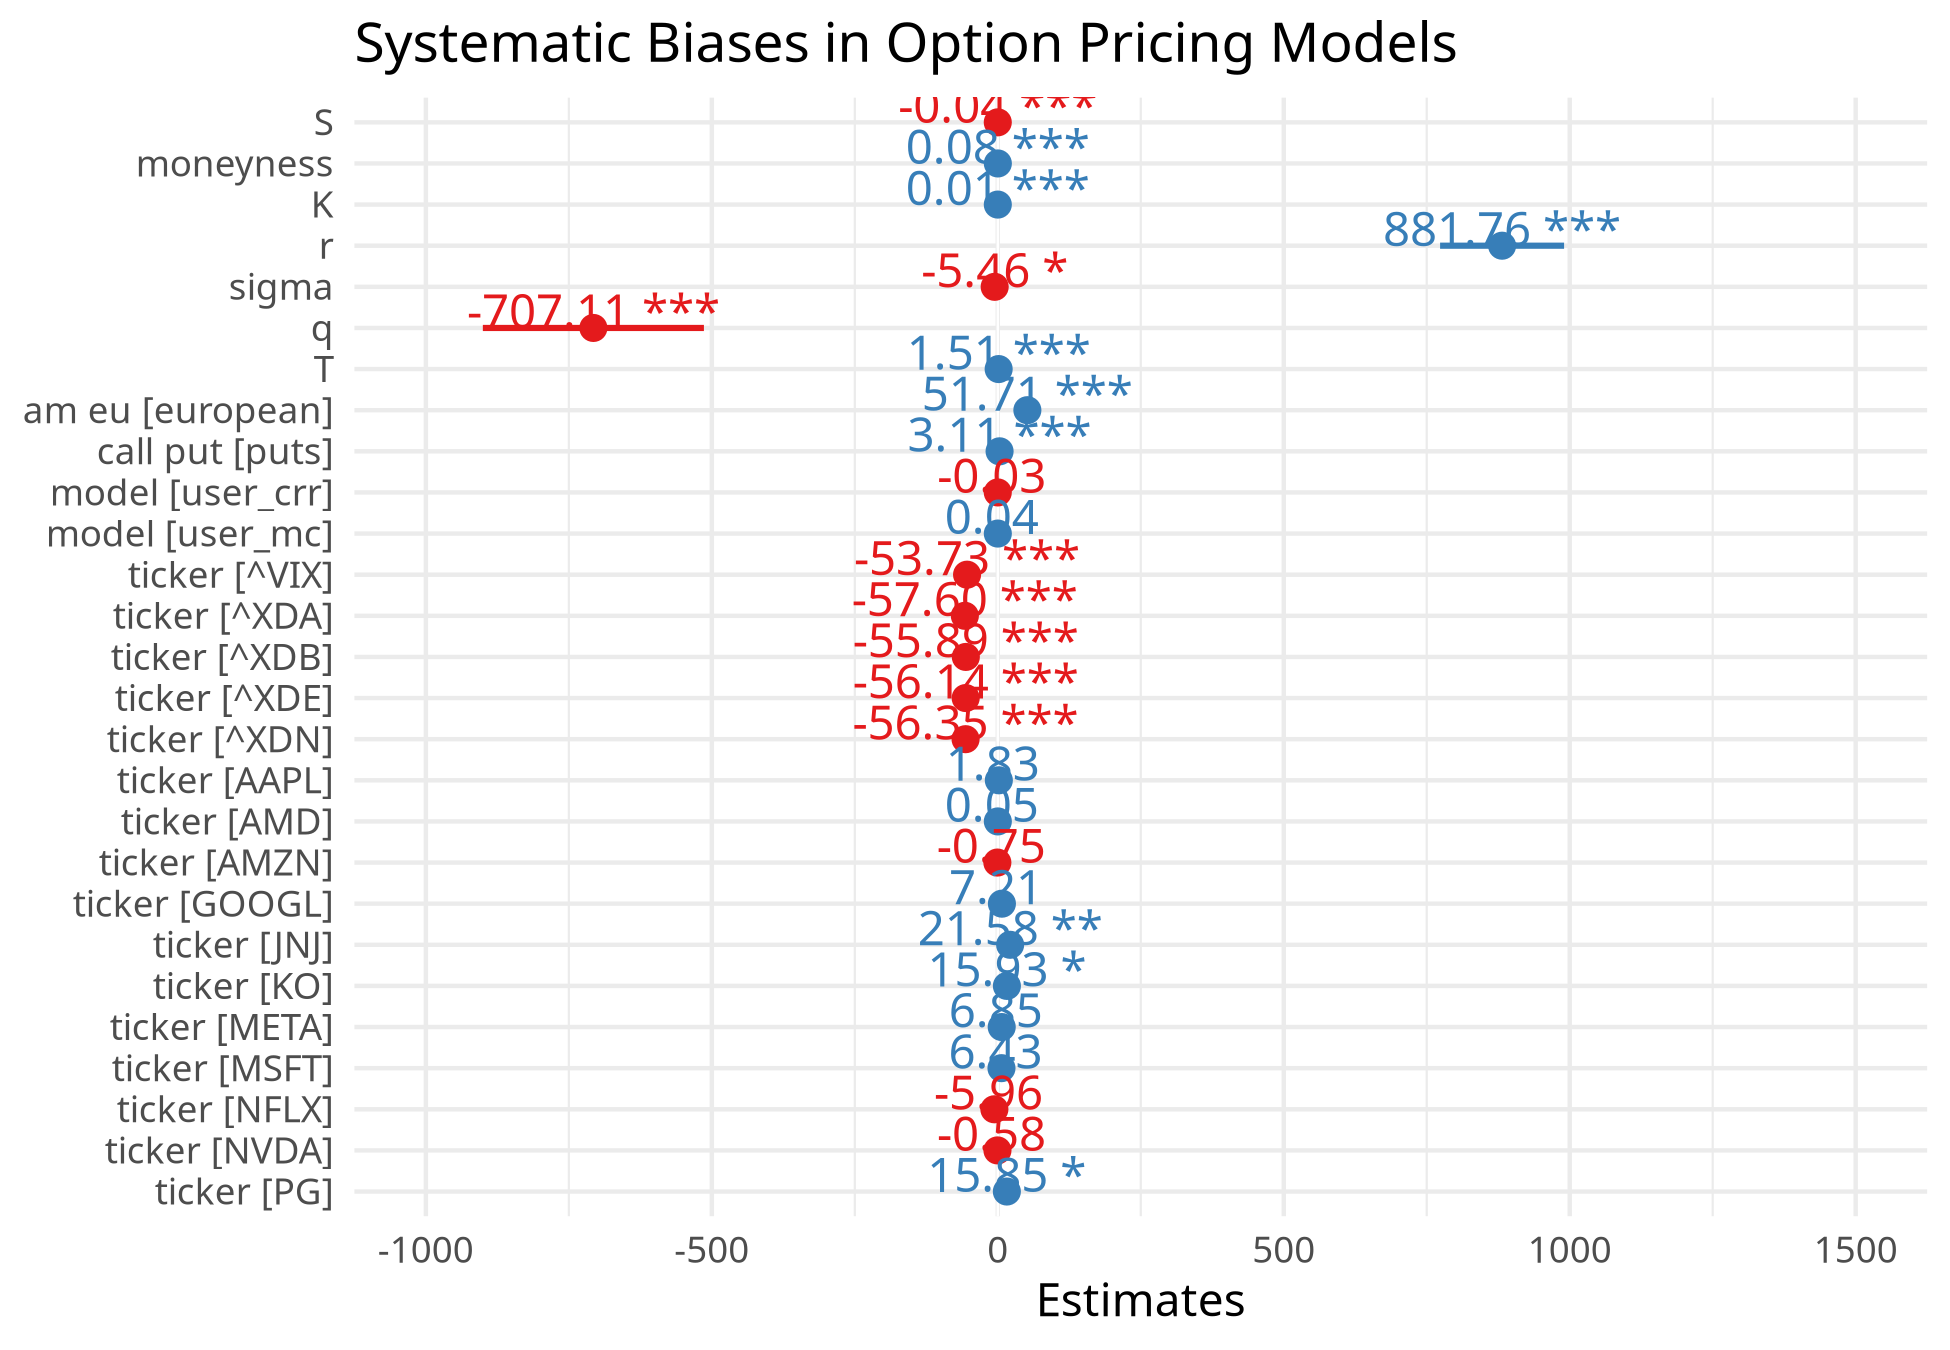
\includegraphics[keepaspectratio]{regression_files/regression_files/figure-latex/rmr_abs_base_bias-1.png}}

\begin{Shaded}
\begin{Highlighting}[]
\NormalTok{train\_data\_abs}\SpecialCharTok{$}\NormalTok{predicted\_error }\OtherTok{\textless{}{-}} \FunctionTok{predict}\NormalTok{(rmr\_absolute)}

\NormalTok{absolute\_hexes }\OtherTok{\textless{}{-}} \FunctionTok{ggplot}\NormalTok{(train\_data\_abs, }\FunctionTok{aes}\NormalTok{(}\AttributeTok{x =}\NormalTok{ predicted\_error, }\AttributeTok{y =}\NormalTok{ pricing\_error)) }\SpecialCharTok{+}
  \FunctionTok{geom\_hex}\NormalTok{(}\AttributeTok{bins =} \DecValTok{70}\NormalTok{) }\SpecialCharTok{+}
  \FunctionTok{scale\_fill\_viridis\_c}\NormalTok{(}\AttributeTok{option =} \StringTok{"plasma"}\NormalTok{) }\SpecialCharTok{+} \CommentTok{\# Cool modern color palette}
  \FunctionTok{geom\_abline}\NormalTok{(}\AttributeTok{slope =} \DecValTok{1}\NormalTok{, }\AttributeTok{intercept =} \DecValTok{0}\NormalTok{, }\AttributeTok{color =} \StringTok{"white"}\NormalTok{, }\AttributeTok{linetype =} \StringTok{"dashed"}\NormalTok{, }\AttributeTok{size =} \DecValTok{1}\NormalTok{) }\SpecialCharTok{+}
  \FunctionTok{theme\_minimal}\NormalTok{() }\SpecialCharTok{+}
  \FunctionTok{labs}\NormalTok{(}
    \AttributeTok{title =} \StringTok{"Model Fit: Actual vs. Predicted Pricing Errors"}\NormalTok{,}
    \AttributeTok{x =} \StringTok{"Predicted Error (Regression Model)"}\NormalTok{,}
    \AttributeTok{y =} \StringTok{"Actual Error (Market {-} Option Model)"}\NormalTok{,}
    \AttributeTok{fill =} \StringTok{"Record Count"}
\NormalTok{  )}

\CommentTok{\#ggsave("\textasciitilde{}/Praxe/bakalarka/figures/absolute\_hexes.png", absolute\_hexes, width = 6, height = 4)}

\NormalTok{absolute\_hexes}
\end{Highlighting}
\end{Shaded}

\pandocbounded{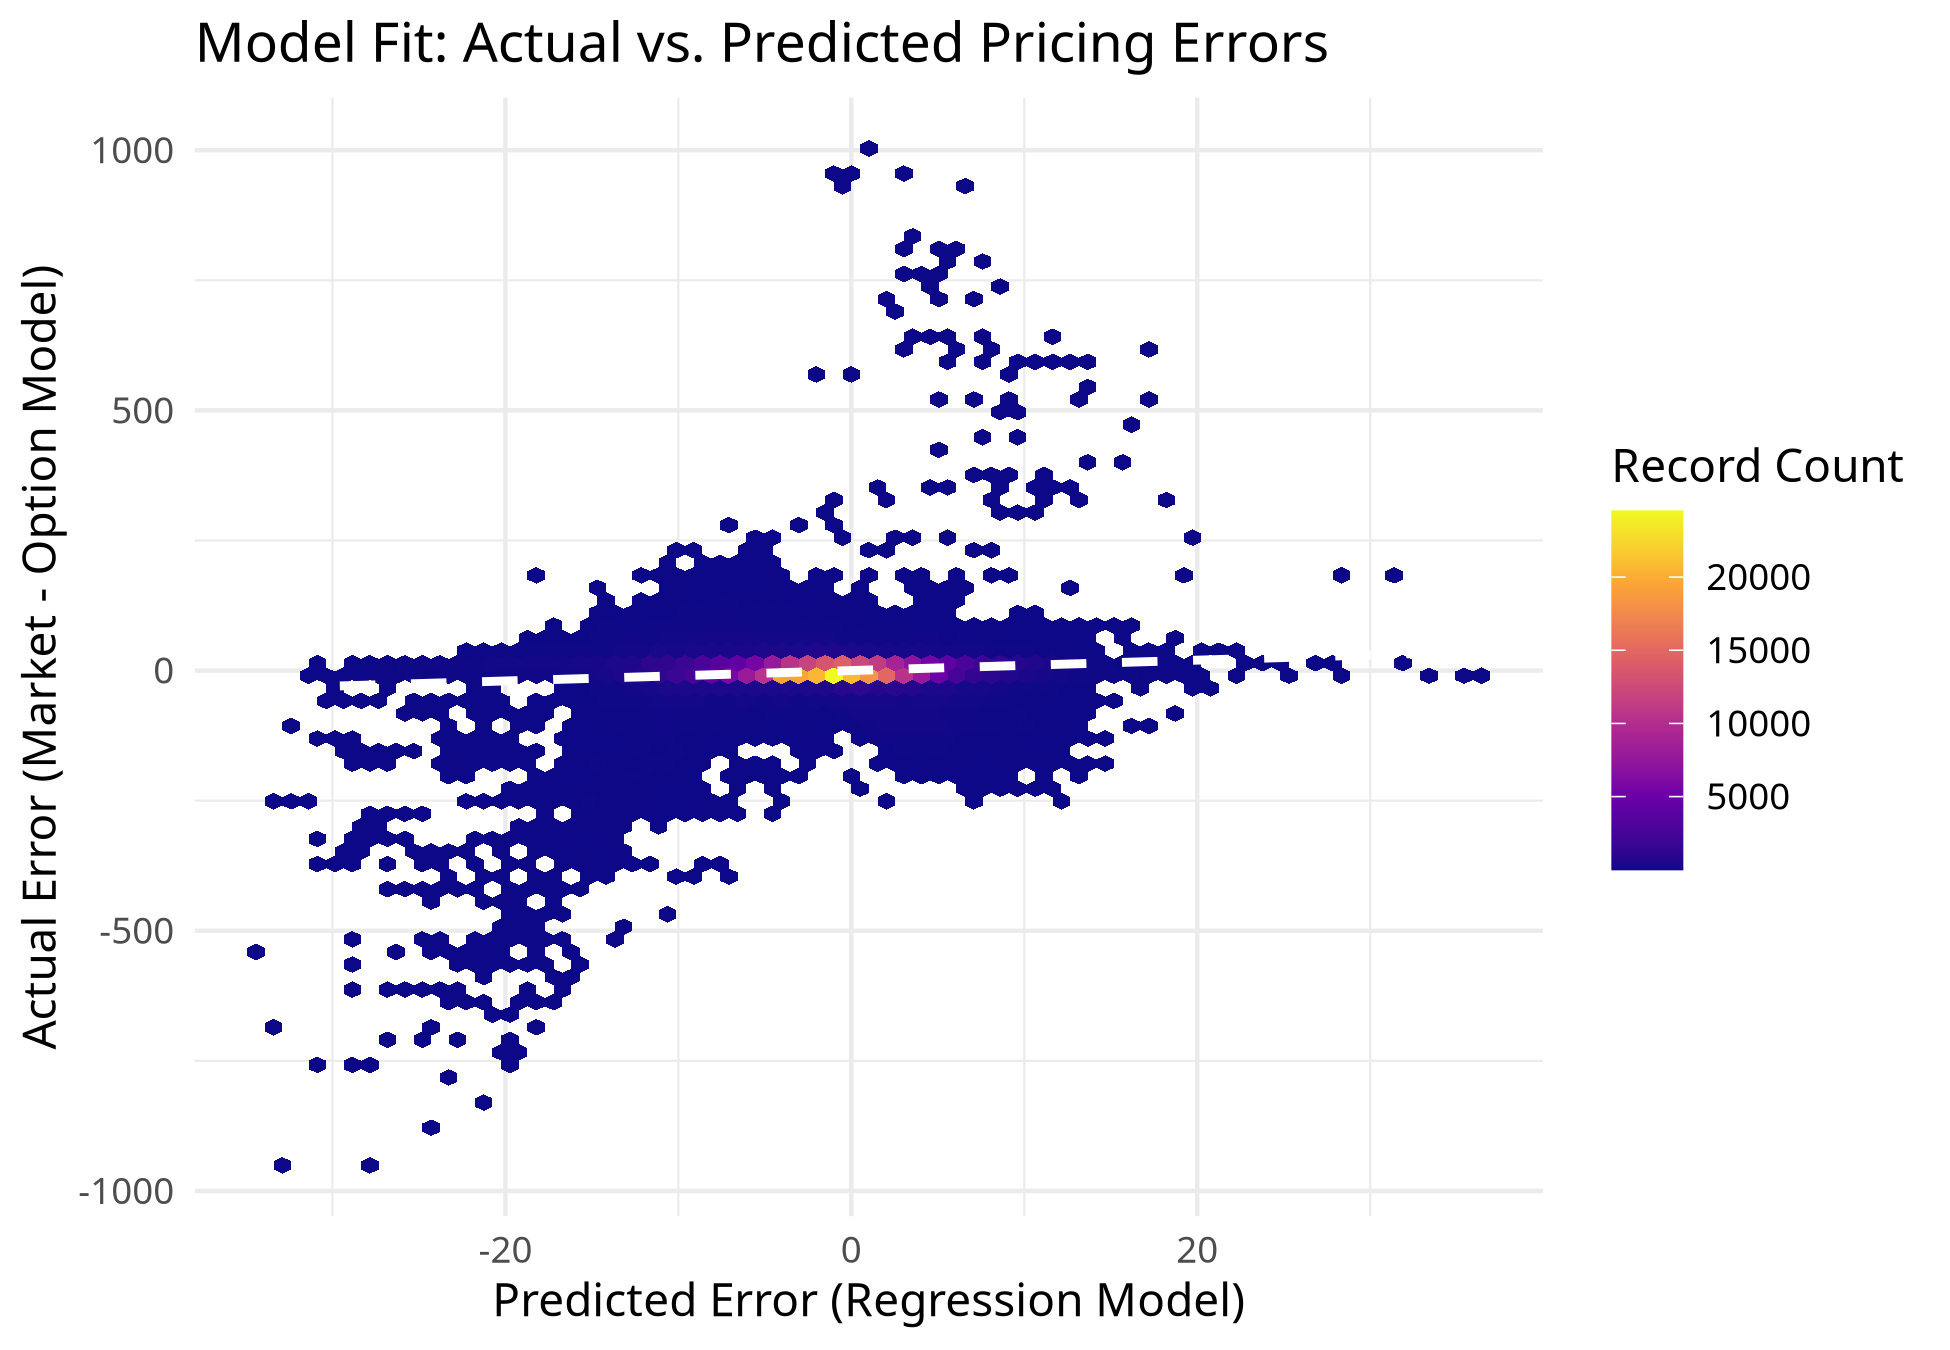
\includegraphics[keepaspectratio]{regression_files/regression_files/figure-latex/rmr_abs_base_predict-1.png}}

\subsection{Relativní}\label{relativnuxed}

\begin{Shaded}
\begin{Highlighting}[]
\NormalTok{df\_relative }\OtherTok{\textless{}{-}}\NormalTok{ df\_doctored }\SpecialCharTok{\%\textgreater{}\%}
  \FunctionTok{pivot\_longer}\NormalTok{(}\AttributeTok{cols =} \FunctionTok{c}\NormalTok{(user\_bs, user\_crr, user\_mc),}
               \AttributeTok{names\_to =} \StringTok{"model"}\NormalTok{,}
               \AttributeTok{values\_to =} \StringTok{"model\_price"}\NormalTok{) }\SpecialCharTok{\%\textgreater{}\%}
  \CommentTok{\#filter(model == "user\_crr") \%\textgreater{}\%}
  \FunctionTok{mutate}\NormalTok{(}\AttributeTok{pricing\_error\_test =}\NormalTok{ (true\_price }\SpecialCharTok{{-}}\NormalTok{ model\_price) }\SpecialCharTok{/}\NormalTok{ true\_price) }\SpecialCharTok{\%\textgreater{}\%}
  \CommentTok{\#mutate(pricing\_error = 2 * (true\_price {-} model\_price) / (true\_price + model\_price)) \%\textgreater{}\%}
  \FunctionTok{mutate}\NormalTok{(}\AttributeTok{pricing\_error =}\NormalTok{ (true\_price }\SpecialCharTok{{-}}\NormalTok{ model\_price) }\SpecialCharTok{/}\NormalTok{ S) }\SpecialCharTok{\%\textgreater{}\%}
  \FunctionTok{filter}\NormalTok{(}\FunctionTok{is.finite}\NormalTok{(pricing\_error)) }\SpecialCharTok{\%\textgreater{}\%}
  \FunctionTok{mutate}\NormalTok{(}\AttributeTok{snapshot\_date =} \FunctionTok{as.Date}\NormalTok{(expiration) }\SpecialCharTok{{-}} \FunctionTok{round}\NormalTok{(T }\SpecialCharTok{*} \DecValTok{365}\NormalTok{)) }\SpecialCharTok{\%\textgreater{}\%}
  \FunctionTok{mutate}\NormalTok{(}\AttributeTok{snapshot\_month =} \FunctionTok{format}\NormalTok{(snapshot\_date, }\StringTok{"\%m"}\NormalTok{))}
\end{Highlighting}
\end{Shaded}

\begin{Shaded}
\begin{Highlighting}[]
\NormalTok{df\_relative\_temp }\OtherTok{\textless{}{-}}\NormalTok{ df\_relative }\CommentTok{\#\%\textgreater{}\% filter(am\_eu == "american" \& call\_put == "calls")}
\NormalTok{train\_indexes }\OtherTok{\textless{}{-}} \FunctionTok{sample}\NormalTok{(}\DecValTok{1}\SpecialCharTok{:}\FunctionTok{nrow}\NormalTok{(df\_relative\_temp), }\AttributeTok{size =} \FloatTok{0.8} \SpecialCharTok{*} \FunctionTok{nrow}\NormalTok{(df\_relative\_temp))}

\NormalTok{train\_data\_rel }\OtherTok{\textless{}{-}}\NormalTok{ df\_relative\_temp[train\_indexes, ]}
\NormalTok{test\_data\_rel }\OtherTok{\textless{}{-}}\NormalTok{ df\_relative\_temp[}\SpecialCharTok{{-}}\NormalTok{train\_indexes, ]}
\end{Highlighting}
\end{Shaded}

\begin{Shaded}
\begin{Highlighting}[]
\FunctionTok{png}\NormalTok{(}\StringTok{"\textasciitilde{}/Praxe/bakalarka/figures/hist\_relative.png"}\NormalTok{, }\AttributeTok{width =} \DecValTok{6}\NormalTok{, }\AttributeTok{height =} \DecValTok{4}\NormalTok{, }\AttributeTok{units =} \StringTok{"in"}\NormalTok{, }\AttributeTok{res =} \DecValTok{300}\NormalTok{)}
\FunctionTok{hist}\NormalTok{(df\_relative\_temp}\SpecialCharTok{$}\NormalTok{pricing\_error, }\AttributeTok{breaks =} \DecValTok{200}\NormalTok{)}
\FunctionTok{dev.off}\NormalTok{()}
\end{Highlighting}
\end{Shaded}

\begin{verbatim}
## png 
##   2
\end{verbatim}

\begin{Shaded}
\begin{Highlighting}[]
\FunctionTok{hist}\NormalTok{(df\_relative\_temp}\SpecialCharTok{$}\NormalTok{pricing\_error, }\AttributeTok{breaks =} \DecValTok{200}\NormalTok{)}
\end{Highlighting}
\end{Shaded}

\pandocbounded{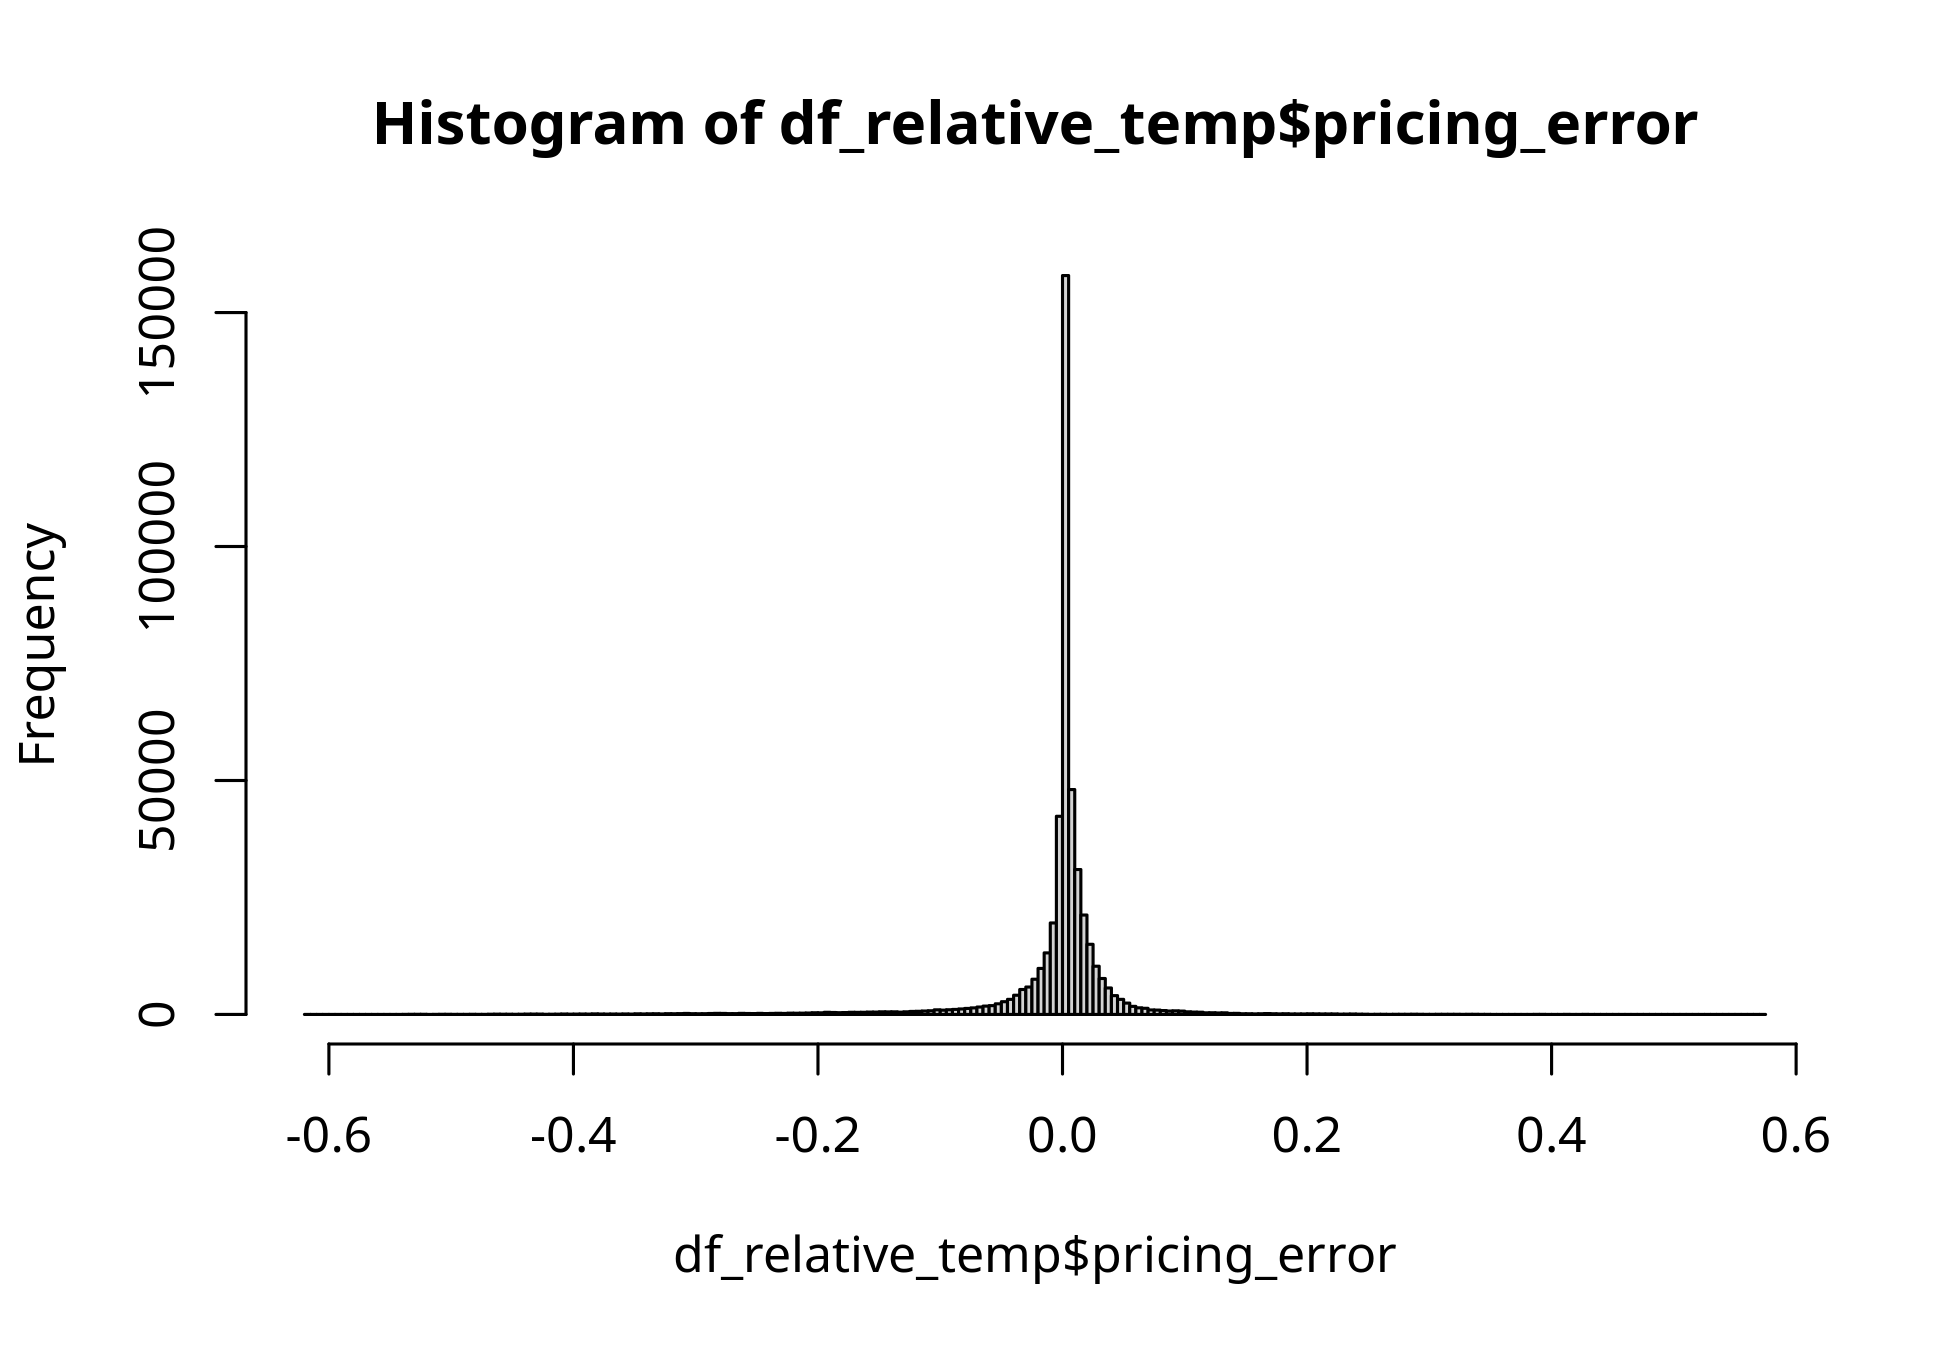
\includegraphics[keepaspectratio]{regression_files/regression_files/figure-latex/unnamed-chunk-7-1.png}}

Distribuce je bimodální: pík u 0 odpovídá přesnému ocenění, pík u 2
odpovídá opcím s odhadovanou cenou blízkou 0. Regresní model tuto
strukturu zohledňuje.

\begin{Shaded}
\begin{Highlighting}[]
\FunctionTok{hist}\NormalTok{(df\_relative\_temp}\SpecialCharTok{$}\NormalTok{pricing\_error\_test, }\AttributeTok{breaks =} \DecValTok{100}\NormalTok{)}
\end{Highlighting}
\end{Shaded}

\pandocbounded{
\includegraphics[keepaspectratio]{regression_files/regression_files/figure-latex/unnamed-chunk-8-1.png}}

\begin{Shaded}
\begin{Highlighting}[]
\NormalTok{train\_data\_rel}\SpecialCharTok{$}\NormalTok{T2 }\OtherTok{\textless{}{-}}\NormalTok{ train\_data\_rel}\SpecialCharTok{$}\NormalTok{T}\SpecialCharTok{\^{}}\DecValTok{2}

\NormalTok{subset\_args }\OtherTok{\textless{}{-}} \FunctionTok{c}\NormalTok{(}
  \StringTok{"S"}\NormalTok{,}
  \StringTok{"K"}\NormalTok{,}
  \CommentTok{\#"r",}
  \StringTok{"sigma"}\NormalTok{,}
  \CommentTok{\#"q",}
  \StringTok{"T"}\NormalTok{,}
  \StringTok{"T2"}\NormalTok{,}
  \CommentTok{\#"am\_eu",}
  \CommentTok{\#"call\_put",}
  \CommentTok{\#"model",}
  \StringTok{"ticker"}\NormalTok{,}
  \StringTok{"snapshot\_month"}
\NormalTok{  )}
\NormalTok{interactions }\OtherTok{\textless{}{-}} \FunctionTok{c}\NormalTok{(}
  \CommentTok{\#"q:am\_eu",}
\NormalTok{)}

\NormalTok{rhs }\OtherTok{\textless{}{-}} \FunctionTok{paste}\NormalTok{(}\FunctionTok{c}\NormalTok{(subset\_args, interactions), }\AttributeTok{collapse =} \StringTok{" + "}\NormalTok{)}
\NormalTok{formula }\OtherTok{\textless{}{-}} \FunctionTok{as.formula}\NormalTok{(}\FunctionTok{paste}\NormalTok{(}\StringTok{"pricing\_error \textasciitilde{} "}\NormalTok{, rhs))}
\CommentTok{\#T\_crr \textless{}{-} lm(pricing\_error \textasciitilde{} T + as.factor(snapshot\_month), data = train\_data)}
\NormalTok{regression\_relative }\OtherTok{\textless{}{-}} \FunctionTok{lm}\NormalTok{(formula, }\AttributeTok{data =}\NormalTok{ train\_data\_rel)}

\FunctionTok{summary}\NormalTok{(regression\_relative)}
\end{Highlighting}
\end{Shaded}

\begin{verbatim}
## 
## Call:
## lm(formula = formula, data = train_data_rel)
## 
## Residuals:
##      Min       1Q   Median       3Q      Max 
## -0.61961 -0.00407  0.00549  0.01396  0.57767 
## 
## Coefficients:
##                    Estimate Std. Error t value Pr(>|t|)    
## (Intercept)       2.481e-02  4.899e-03   5.063 4.12e-07 ***
## S                 9.588e-06  1.865e-06   5.139 2.76e-07 ***
## K                -1.652e-05  3.940e-07 -41.926  < 2e-16 ***
## sigma            -5.685e-02  3.429e-03 -16.581  < 2e-16 ***
## T                -5.366e-03  3.864e-04 -13.888  < 2e-16 ***
## T2                4.085e-03  1.615e-04  25.287  < 2e-16 ***
## ticker^VIX       -1.514e-02  6.857e-03  -2.208  0.02724 *  
## ticker^XDA       -3.370e-02  7.725e-03  -4.363 1.28e-05 ***
## ticker^XDB       -4.759e-03  6.875e-03  -0.692  0.48878    
## ticker^XDE       -1.737e-02  5.914e-03  -2.936  0.00332 ** 
## ticker^XDN       -8.853e-03  6.458e-03  -1.371  0.17039    
## tickerAAPL       -1.254e-02  4.568e-03  -2.746  0.00603 ** 
## tickerAMD         2.852e-03  4.944e-03   0.577  0.56402    
## tickerAMZN       -3.442e-03  4.686e-03  -0.734  0.46271    
## tickerGOOGL       1.565e-03  4.475e-03   0.350  0.72657    
## tickerJNJ        -1.844e-02  4.576e-03  -4.030 5.59e-05 ***
## tickerKO         -1.427e-02  4.861e-03  -2.936  0.00333 ** 
## tickerMETA       -4.635e-03  4.008e-03  -1.157  0.24740    
## tickerMSFT       -1.191e-02  4.267e-03  -2.791  0.00526 ** 
## tickerNFLX       -1.598e-02  4.936e-03  -3.237  0.00121 ** 
## tickerNVDA        3.868e-03  4.841e-03   0.799  0.42429    
## tickerPG         -1.100e-02  4.739e-03  -2.320  0.02032 *  
## tickerTSLA       -3.782e-04  4.631e-03  -0.082  0.93491    
## snapshot_month02  2.101e-05  2.552e-04   0.082  0.93440    
## snapshot_month03  2.334e-03  2.772e-04   8.419  < 2e-16 ***
## snapshot_month05  4.106e-03  3.321e-04  12.365  < 2e-16 ***
## ---
## Signif. codes:  0 '***' 0.001 '**' 0.01 '*' 0.05 '.' 0.1 ' ' 1
## 
## Residual standard error: 0.05419 on 375336 degrees of freedom
## Multiple R-squared:  0.05632,    Adjusted R-squared:  0.05626 
## F-statistic:   896 on 25 and 375336 DF,  p-value: < 2.2e-16
\end{verbatim}

\begin{Shaded}
\begin{Highlighting}[]
\FunctionTok{png}\NormalTok{(}\StringTok{"\textasciitilde{}/Praxe/bakalarka/figures/relative\_basic.png"}\NormalTok{, }\AttributeTok{width =} \DecValTok{6}\NormalTok{, }\AttributeTok{height =} \DecValTok{4}\NormalTok{, }\AttributeTok{units =} \StringTok{"in"}\NormalTok{, }\AttributeTok{res =} \DecValTok{300}\NormalTok{)}
\FunctionTok{par}\NormalTok{(}\AttributeTok{mfrow =} \FunctionTok{c}\NormalTok{(}\DecValTok{2}\NormalTok{, }\DecValTok{2}\NormalTok{))}
\FunctionTok{plot}\NormalTok{(regression\_relative)}
\FunctionTok{dev.off}\NormalTok{()}
\end{Highlighting}
\end{Shaded}

\begin{verbatim}
## png 
##   2
\end{verbatim}

\begin{Shaded}
\begin{Highlighting}[]
\FunctionTok{par}\NormalTok{(}\AttributeTok{mfrow =} \FunctionTok{c}\NormalTok{(}\DecValTok{2}\NormalTok{, }\DecValTok{2}\NormalTok{))}
\FunctionTok{plot}\NormalTok{(regression\_relative)}
\end{Highlighting}
\end{Shaded}

\pandocbounded{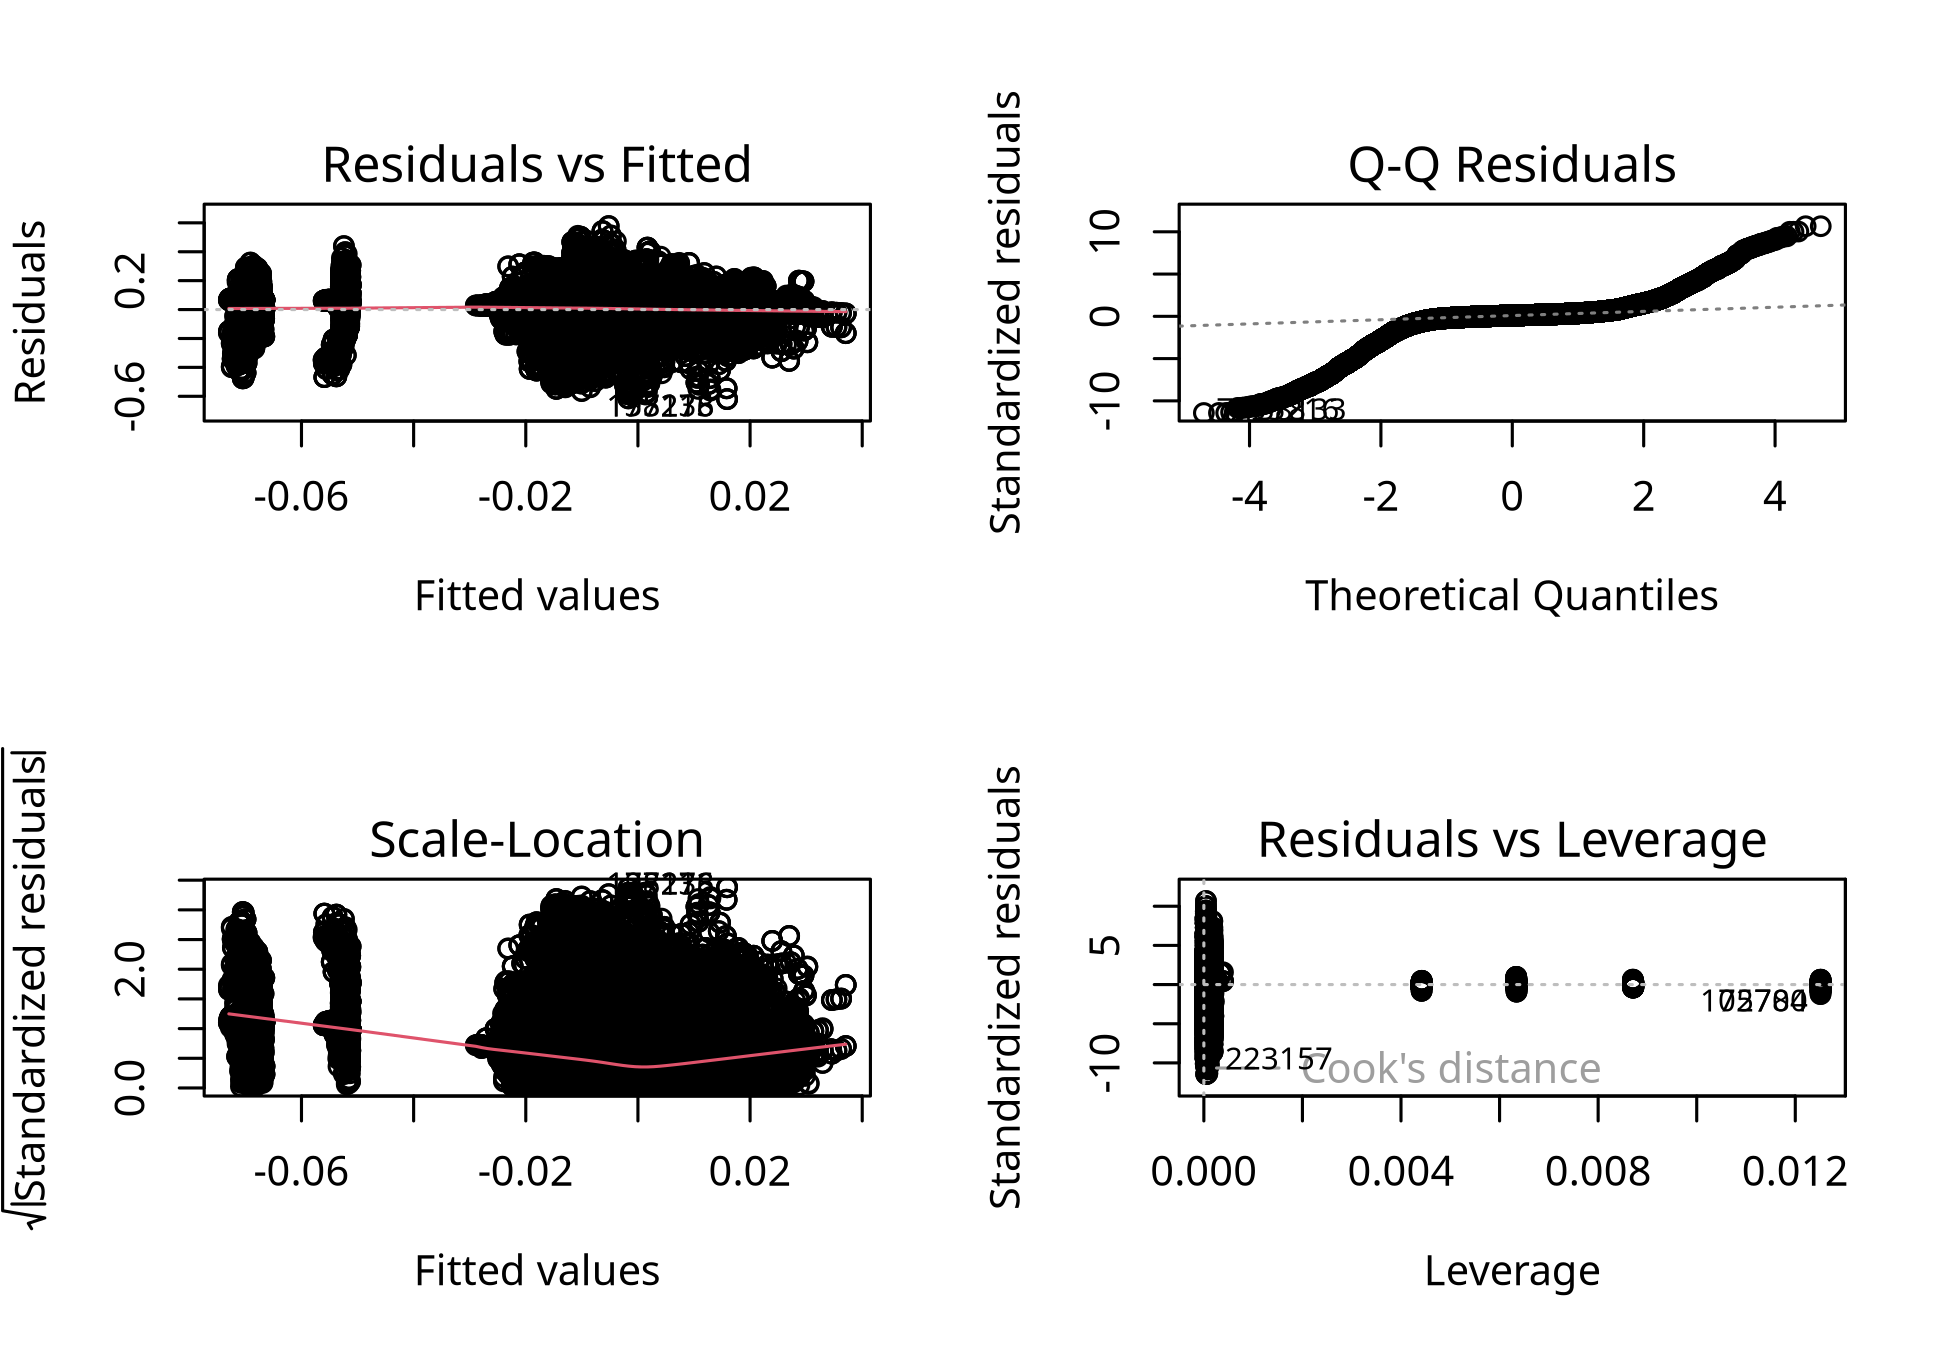
\includegraphics[keepaspectratio]{regression_files/regression_files/figure-latex/plot-1.png}}

\begin{Shaded}
\begin{Highlighting}[]
\FunctionTok{par}\NormalTok{(}\AttributeTok{mfrow =} \FunctionTok{c}\NormalTok{(}\DecValTok{1}\NormalTok{, }\DecValTok{1}\NormalTok{))}
\end{Highlighting}
\end{Shaded}

\subsubsection{Předpoklady}\label{pux159edpoklady-1}

Kontrola homoscedasticity:

\begin{Shaded}
\begin{Highlighting}[]
\FunctionTok{bptest}\NormalTok{(regression\_relative)}
\end{Highlighting}
\end{Shaded}

\begin{verbatim}
## 
##  studentized Breusch-Pagan test
## 
## data:  regression_relative
## BP = 18631, df = 25, p-value < 2.2e-16
\end{verbatim}

Dle výsledků Breuschova-Paganova testu (p \textless{} 0.05) zamítáme
null hypotézu → je přítomná heteroskedasticita.

Kontrola autokorelace:

\begin{Shaded}
\begin{Highlighting}[]
\FunctionTok{dwtest}\NormalTok{(regression\_relative)}
\end{Highlighting}
\end{Shaded}

\begin{verbatim}
## 
##  Durbin-Watson test
## 
## data:  regression_relative
## DW = 2.0014, p-value = 0.6702
## alternative hypothesis: true autocorrelation is greater than 0
\end{verbatim}

Dle výsledku Durbinova-Watsonova testu je přítomná autokorelace. Opce ze
stejného tickeru jsou navzájem závislé.

Použijeme cluster-robust standardní chyby (cluster na ticker), které
opravují heteroskedasticitu i autokorelací zároveň:

Kontrola multikolinearity:

\begin{Shaded}
\begin{Highlighting}[]
\FunctionTok{vif}\NormalTok{(regression\_relative, }\AttributeTok{type =} \StringTok{"predictor"}\NormalTok{)}
\end{Highlighting}
\end{Shaded}

\begin{verbatim}
## GVIFs computed for predictors
\end{verbatim}

\begin{verbatim}
##                        GVIF Df GVIF^(1/(2*Df)) Interacts With
## S                255.232673  1       15.976003           --  
## K                 10.911433  1        3.303246           --  
## sigma             62.725842  1        7.919965           --  
## T                  9.964841  1        3.156714           --  
## T2                 9.748495  1        3.122258           --  
## ticker         14276.305338 17        1.324935           --  
## snapshot_month     2.911806  3        1.194979           --  
##                                       Other Predictors
## S              K, sigma, T, T2, ticker, snapshot_month
## K              S, sigma, T, T2, ticker, snapshot_month
## sigma              S, K, T, T2, ticker, snapshot_month
## T              S, K, sigma, T2, ticker, snapshot_month
## T2              S, K, sigma, T, ticker, snapshot_month
## ticker              S, K, sigma, T, T2, snapshot_month
## snapshot_month              S, K, sigma, T, T2, ticker
\end{verbatim}

\subsubsection{LMER model -
základní}\label{lmer-model---zuxe1kladnuxed-1}

\begin{Shaded}
\begin{Highlighting}[]
\NormalTok{subset\_args }\OtherTok{\textless{}{-}} \FunctionTok{c}\NormalTok{(}
  \StringTok{"S"}\NormalTok{,}
  \StringTok{"moneyness"}\NormalTok{,}
  \StringTok{"K"}\NormalTok{,}
  \StringTok{"r"}\NormalTok{,}
  \StringTok{"sigma"}\NormalTok{,}
  \StringTok{"q"}\NormalTok{,}
  \StringTok{"T"}\NormalTok{,}
  \StringTok{"am\_eu"}\NormalTok{,}
  \StringTok{"call\_put"}\NormalTok{,}
  \StringTok{"model"}\NormalTok{,}
  \StringTok{"ticker"}
\NormalTok{  )}
\NormalTok{interactions }\OtherTok{\textless{}{-}} \FunctionTok{c}\NormalTok{(}
  \StringTok{"q:am\_eu"}\NormalTok{,}
  \CommentTok{\#"(1 | option\_id)",}
  \StringTok{"(1 | ticker)"}\NormalTok{,}
  \StringTok{"(1 | snapshot\_month)"}
\NormalTok{)}

\NormalTok{rhs }\OtherTok{\textless{}{-}} \FunctionTok{paste}\NormalTok{(}\FunctionTok{c}\NormalTok{(subset\_args, interactions), }\AttributeTok{collapse =} \StringTok{" + "}\NormalTok{)}
\NormalTok{formula }\OtherTok{\textless{}{-}} \FunctionTok{as.formula}\NormalTok{(}\FunctionTok{paste}\NormalTok{(}\StringTok{"pricing\_error \textasciitilde{} "}\NormalTok{, rhs))}

\NormalTok{rmr\_relative }\OtherTok{\textless{}{-}} \FunctionTok{lmer}\NormalTok{(formula, }\AttributeTok{data =}\NormalTok{ train\_data\_rel)}
\end{Highlighting}
\end{Shaded}

\begin{verbatim}
## fixed-effect model matrix is rank deficient so dropping 2 columns / coefficients
\end{verbatim}

\begin{verbatim}
## Warning: Some predictor variables are on very different scales: consider rescaling. 
## You may also use (g)lmerControl(autoscale = TRUE) to improve numerical stability.
\end{verbatim}

\begin{Shaded}
\begin{Highlighting}[]
\FunctionTok{summary}\NormalTok{(rmr\_relative)}
\end{Highlighting}
\end{Shaded}

\begin{verbatim}
## Linear mixed model fit by REML ['lmerMod']
## Formula: pricing_error ~ S + moneyness + K + r + sigma + q + T + am_eu +  
##     call_put + model + ticker + q:am_eu + (1 | ticker) + (1 |  
##     snapshot_month)
##    Data: train_data_rel
## 
## REML criterion at convergence: -1131942
## 
## Scaled residuals: 
##      Min       1Q   Median       3Q      Max 
## -11.8145  -0.1034   0.1061   0.2862  10.6800 
## 
## Random effects:
##  Groups         Name        Variance  Std.Dev. 
##  ticker         (Intercept) 1.482e-04 0.0121754
##  snapshot_month (Intercept) 6.883e-07 0.0008296
##  Residual                   2.867e-03 0.0535455
## Number of obs: 375362, groups:  ticker, 18; snapshot_month, 4
## 
## Fixed effects:
##                 Estimate Std. Error t value
## (Intercept)   -6.722e-02  1.273e-02  -5.279
## S              1.379e-05  1.819e-06   7.582
## moneyness     -1.111e-05  1.086e-05  -1.023
## K             -2.249e-05  4.027e-07 -55.852
## r              2.730e+00  8.555e-02  31.909
## sigma         -5.975e-02  3.319e-03 -18.006
## q             -1.210e+00  1.534e-01  -7.890
## T              4.456e-03  1.260e-04  35.373
## am_eueuropean  3.599e-03  1.779e-02   0.202
## call_putputs  -1.658e-02  1.778e-04 -93.250
## modeluser_crr -4.731e-05  2.140e-04  -0.221
## modeluser_mc   4.068e-05  2.141e-04   0.190
## ticker^VIX    -1.793e-02  1.844e-02  -0.972
## ticker^XDA    -4.762e-02  1.882e-02  -2.530
## ticker^XDB    -2.301e-03  1.850e-02  -0.124
## ticker^XDE    -2.336e-02  1.817e-02  -1.286
## ticker^XDN    -1.993e-02  1.835e-02  -1.086
## tickerAAPL    -8.337e-03  1.726e-02  -0.483
## tickerAMD      2.598e-03  1.723e-02   0.151
## tickerAMZN    -4.290e-03  1.724e-02  -0.249
## tickerGOOGL    5.922e-03  1.726e-02   0.343
## tickerJNJ      2.075e-02  1.803e-02   1.151
## tickerKO       2.111e-02  1.789e-02   1.180
## tickerMETA    -8.708e-04  1.725e-02  -0.050
## tickerMSFT    -2.465e-03  1.730e-02  -0.142
## tickerNFLX    -1.786e-02  1.724e-02  -1.036
## tickerNVDA     3.407e-03  1.723e-02   0.198
## tickerPG       2.077e-02  1.777e-02   1.169
\end{verbatim}

\begin{verbatim}
## 
## Correlation matrix not shown by default, as p = 28 > 12.
## Use print(x, correlation=TRUE)  or
##     vcov(x)        if you need it
\end{verbatim}

\begin{verbatim}
## fit warnings:
## fixed-effect model matrix is rank deficient so dropping 2 columns / coefficients
## Some predictor variables are on very different scales: consider rescaling. 
## You may also use (g)lmerControl(autoscale = TRUE) to improve numerical stability.
\end{verbatim}

\begin{Shaded}
\begin{Highlighting}[]
\FunctionTok{r2}\NormalTok{(rmr\_relative)}
\end{Highlighting}
\end{Shaded}

\begin{verbatim}
## Warning: Can't compute random effect variances. Some variance components equal
##   zero. Your model may suffer from singularity (see `?lme4::isSingular`
##   and `?performance::check_singularity`).
##   Decrease the `tolerance` level to force the calculation of random effect
##   variances, or impose priors on your random effects parameters (using
##   packages like `brms` or `glmmTMB`).
\end{verbatim}

\begin{verbatim}
## Random effect variances not available. Returned R2 does not account for random effects.
\end{verbatim}

\begin{verbatim}
## # R2 for Mixed Models
## 
##   Conditional R2: NA
##      Marginal R2: 0.079
\end{verbatim}

\begin{Shaded}
\begin{Highlighting}[]
\NormalTok{relative\_bias\_plot }\OtherTok{\textless{}{-}} \FunctionTok{plot\_model}\NormalTok{(rmr\_relative, }\AttributeTok{type =} \StringTok{"est"}\NormalTok{, }\AttributeTok{show.values =} \ConstantTok{TRUE}\NormalTok{, }\AttributeTok{value.offset =}\NormalTok{ .}\DecValTok{4}\NormalTok{) }\SpecialCharTok{+}
  \FunctionTok{theme\_minimal}\NormalTok{() }\SpecialCharTok{+}
  \FunctionTok{labs}\NormalTok{(}\AttributeTok{title =} \StringTok{"Systematic Biases in Option Pricing Models"}\NormalTok{)}

\CommentTok{\#ggsave("\textasciitilde{}/Praxe/bakalarka/figures/relative\_bias.png", relative\_bias\_plot, width = 6, height = 4)}

\NormalTok{relative\_bias\_plot}
\end{Highlighting}
\end{Shaded}

\pandocbounded{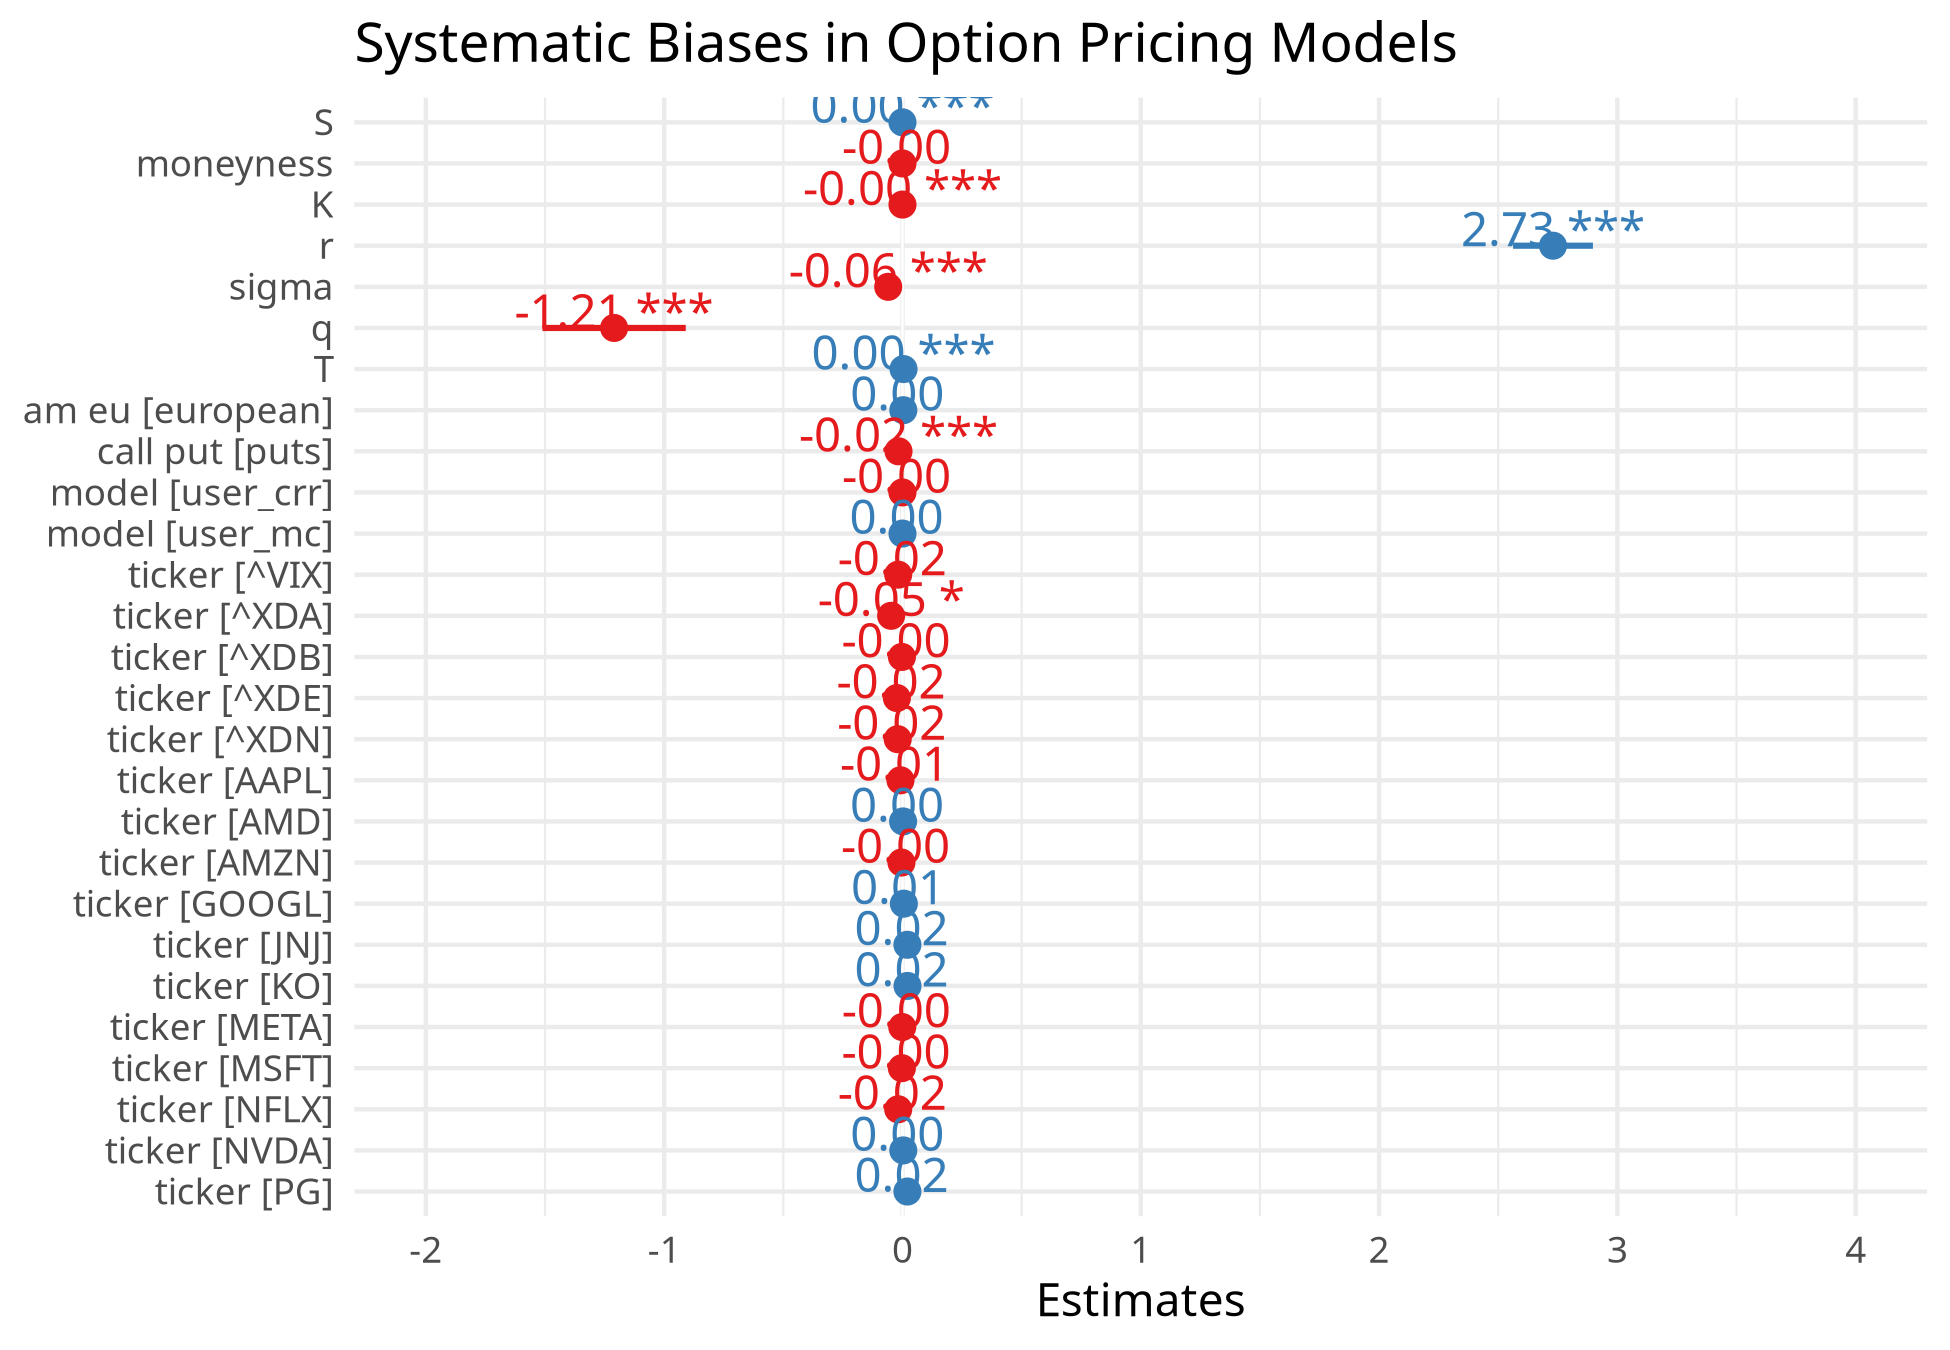
\includegraphics[keepaspectratio]{regression_files/regression_files/figure-latex/unnamed-chunk-11-1.png}}

\begin{Shaded}
\begin{Highlighting}[]
\NormalTok{train\_data\_rel}\SpecialCharTok{$}\NormalTok{predicted\_error }\OtherTok{\textless{}{-}} \FunctionTok{predict}\NormalTok{(rmr\_relative)}

\NormalTok{relative\_hexes }\OtherTok{\textless{}{-}} \FunctionTok{ggplot}\NormalTok{(train\_data\_rel, }\FunctionTok{aes}\NormalTok{(}\AttributeTok{x =}\NormalTok{ predicted\_error, }\AttributeTok{y =}\NormalTok{ pricing\_error)) }\SpecialCharTok{+}
  \FunctionTok{geom\_hex}\NormalTok{(}\AttributeTok{bins =} \DecValTok{70}\NormalTok{) }\SpecialCharTok{+}
  \FunctionTok{scale\_fill\_viridis\_c}\NormalTok{(}\AttributeTok{option =} \StringTok{"plasma"}\NormalTok{) }\SpecialCharTok{+} \CommentTok{\# Cool modern color palette}
  \FunctionTok{geom\_abline}\NormalTok{(}\AttributeTok{slope =} \DecValTok{1}\NormalTok{, }\AttributeTok{intercept =} \DecValTok{0}\NormalTok{, }\AttributeTok{color =} \StringTok{"white"}\NormalTok{, }\AttributeTok{linetype =} \StringTok{"dashed"}\NormalTok{, }\AttributeTok{size =} \DecValTok{1}\NormalTok{) }\SpecialCharTok{+}
  \FunctionTok{theme\_minimal}\NormalTok{() }\SpecialCharTok{+}
  \FunctionTok{labs}\NormalTok{(}
    \AttributeTok{title =} \StringTok{"Model Fit: Actual vs. Predicted Pricing Errors"}\NormalTok{,}
    \AttributeTok{x =} \StringTok{"Predicted Error (Regression Model)"}\NormalTok{,}
    \AttributeTok{y =} \StringTok{"Actual Error (Market {-} Option Model)"}\NormalTok{,}
    \AttributeTok{fill =} \StringTok{"Record Count"}
\NormalTok{  )}

\CommentTok{\#ggsave("\textasciitilde{}/Praxe/bakalarka/figures/relative\_predict.png", relative\_hexes, width = 6, height = 4)}

\NormalTok{relative\_hexes}
\end{Highlighting}
\end{Shaded}

\pandocbounded{
\includegraphics[keepaspectratio]{regression_files/regression_files/figure-latex/rmr_rel_base_predict-1.png}}

\end{document}
